\chapter{Knowledge Base Design: Rules}

\hspace{0.3in}The eTourplan rule system has three distinct top-level operations as shown in Figure 5.1. Using the fact base structured with ontologies described in Chapter Four, the current Chapter examines the main functionalities that we have implemented using rules in POSL syntax. The classification of these operations is as follows: 

\begin{figure}
\begin{center}
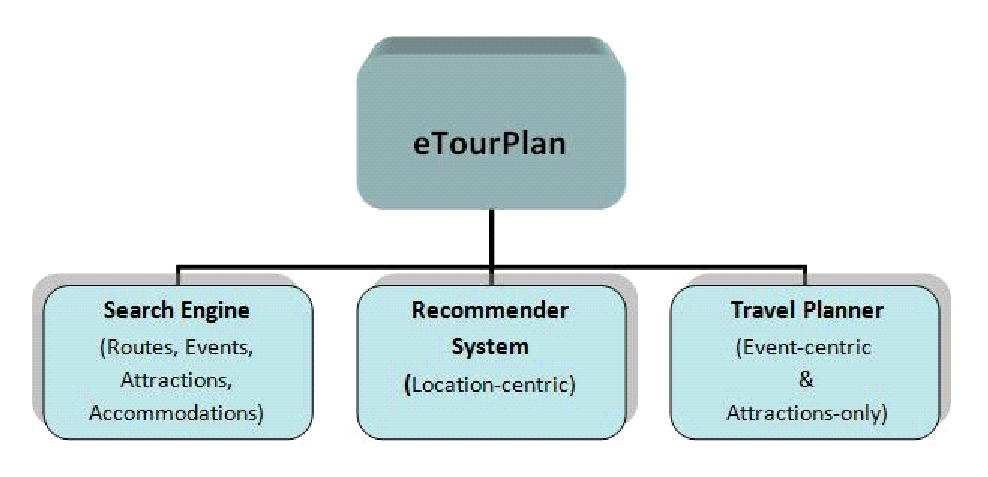
\includegraphics[width=13cm, height=6.5cm]{eTourPlan}
\caption {The top-level architecture of the eTourPlan}
\label{fig:Fig5.1}
\end{center}
\end{figure} 


\begin{itemize}
\item \textbf{Search Engine}: Our KB consists of facts about the five main subdomains of tourism: events, attractions, accommodations, transportation, and regions. This KB can be used for a semantic information search on these subdomains. For example, users can query for detailed information about any specific province, event, attraction, accommodation, or route. The search engine allows parametric searches of information based on a user's preferred parameters, such as search by name, theme, or location. Another flexibility offered to our users is that they can find information about any tourist entity, at any sublevel of the country, from the largest search space (country) to the lowest level (subblock). The details of search options are discussed in Section 5.2.

\item \textbf{Recommender System}: The FOAF-like profiles of neighbouring provinces in our KB are linked together from a touristic point of view as shown in Section 4.2.1. This relation among the provinces in our KB allows us to provide system recommendation of route and activity by chaining through one province to the next related province. It basically uses the FOAF concept to provide location-centric recommendations of activities. The two modes of the location-centric travel recommender are discussed in Section 5.2.4. 

\item \textbf{Travel Planner}: The main travel planner rule system integrates the functionalities of the search and location-centric recommender subsystems. In order to build a travel planner, we need to take into account crucial constraints such as time and distance. The planner employs the various predicates for different operations such as date validation, route finding, and event search in the KB. We have implemented two modes of planning, event-centric and attraction-only planning (cf. Table 2.1 in Section 2.1). The event-centric planning is based on a temporal-geographic search criterion. The FOAF relation between attractions is used as the primary basis for planning a travel in attraction-only mode. These are discussed in detail in Section 5.3.

\end{itemize}
%\hspace{0.3in} In this thesis, we have only considered a small cost measure for the accommodation subdomain. A similar approach can be used to include the total cost of the travel but it is not discussed in this thesis and left as future work. 

\hspace{0.3in}Our eTourPlan rule system offers the following options to our users:

\begin{itemize}
\item Parametric search of tourist information
\item System route planning based on province profiles
\item Route planning for user-preferred provinces 
\item Location-centric recommendation by the system
\item Location-centric recommendation for user-preferred provinces
\item Attraction-only travel planning
\item Event-centric travel planning with attraction recommendations 
\end{itemize}

\hspace{0.3in} Following the design and structure of the KB facts described in Chapter Four, we now discuss the rule subsystems that operate on top of these facts. In Section 5.1, we discuss two main auxiliary rules, for the administrative partonomy and route computation. We discuss the differences and the interrelations between a partonomy and a taxonomy, both of which are used for defining the Regions subdomain. This is followed by a section discussing the route computation rule subsystem. Each of the top-level rule subsystems (cf. Figure 5.1) that are integrated in our eTourPlan prototype are discussed in Section 5.2. Finally, we describe our main travel planning rule system in Section 5.3.

\section{Auxiliary Rules}
\subsection{Partonomy rules}
\hspace{0.3in}Partonomy is a classification system based on the partOf relation between subparts and superparts. We did not implement a RDFS ontology for the Regions subdomain because the partOf relation is different from the subClassOf property that is used in the RDFS for the rest of the subdomains discussed earlier (in Section 4.2). The Regions subdomain is instead structured in our KB using partonomy rules. The superpart (country) is categorized into four subregions: the Eastern\_region, the Central\_region, the Western\_region, and the Southern\_region (There is no Northern\_region since northern Bhutan is covered with mountains). These subregions are classified into provinces, and provinces in turn are subclassified into blocks, which are further classified into four subblock types: city, town, village, or place. These subblocks, then, contain attractions, event locations, and accommodations, which are described as their elements. We will now look at two different approaches to define the partonomy of a region.

\subsubsection{Classification of Regions}

\hspace{0.3in}Before discussing the classification of regions using partonomy rules, we would like to briefly discuss the distinction and the interrelation between a partonomy and a taxonomy. A taxonomy is a hierarchical classification of representing a partial order classes at different levels of abstraction. A taxonomy can be regarded as an ``order-sorted type hierarchy". A partonomy, as previously discussed, is a hierarchical division according of superparts into subparts. Both classifications are asymmetric as well as transitive, and both can form hierarchies \cite{MT:06}. 

\hspace{0.3in}However, there are several differences between partonomy and taxonomy classifications. First, since a taxonomy is the hierarchy of classes whereby lower levels are related to upper levels by inclusion, the subclasses generally allow the inference of properties from superclasses. Part-of relations do not support such an inheritance; i.e., properties of the whole are not necessarily also properties of its parts. Second, a taxonomy describes the division of a set of objects according to various categories, each one containing a set of objects. A partonomy, on the other hand, describes the part of an object with its subparts. Tversky in \cite{TB:90} said that ``A partonomic analysis reveals subcomponents and the relations among them, whereas a taxonomic investigation reveals features shared by a number of instances and their range of variability." 

%\hspace{0.3in}He continues, ``Partonomy is a consequence of an analytic attitude, of a top-down investigation, in which a whole is decomposed into parts on the basis of relative integrality". 

\hspace{0.3in} A partonomy is a one-to-many relation. On the other hand, a taxonomy can be either a one-to-many or a many-to-many relation. In most cases, a taxonomy is the product of a bottom-up investigation, in which objects are grouped on the basis of common and distinctive features \cite{MT:06}

\hspace{0.3in}Both taxonomic and partonomic knowledge are essential parts of our KB, and the usefulness of both of these forms of knowledge are shown together in the implementation of the Regions subdomain. We present an administrative subdivision of a country (Figure 5.2) implemented in POSL syntax: domain-specific and general partonomy rules.\\

\begin{figure}
\begin{center}
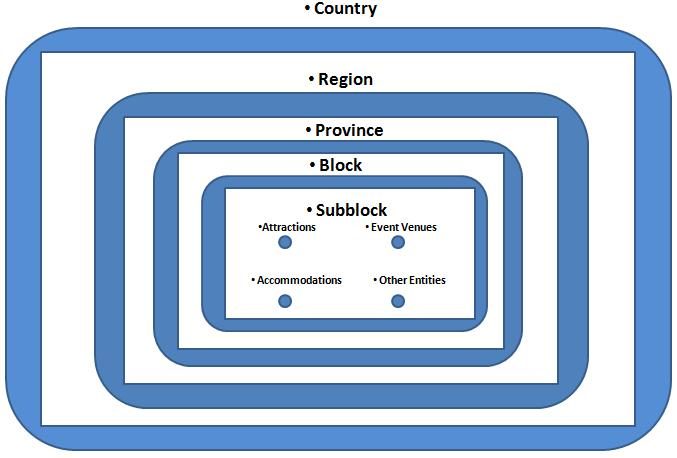
\includegraphics[width=15.5cm, height=9.5cm]{partonomy}
\caption {Subparts of a Country}
\label{fig:Fig5.1}
\end{center}
\end{figure}


\subsubsection{Domain-Specific Partonomy Rule}

\hspace{0.3in}An example of the partonomy of Bhutan dividing the country into  smaller regions and further locating its smallest instances (attractions, event locations, and accommodations) is shown in Figure 5.3. Protege, an ontology editor and knowledge acquisition system, is used here only for visual demonstration purposes, to illustrate the partonomy of the country. We can see that the lowest node of the tree are tourist entities. For example, in Figure 5.3, ``Tashichoedzong" is an attraction of type ``fortress" located in the subblock ``Jongshina" of type ``town" under the block ``Chang" in the province ''Thimphu", which is located in the western region of Bhutan. The POSL representation of this example is shown below, along  with some other sample facts. The subpart representation of a country is described with an n-ary predicate with respect to a location of an attraction. This is a domain-specific approach to represent the partOf relationships of a country. 
\\
\begin{figure}
\begin{center}
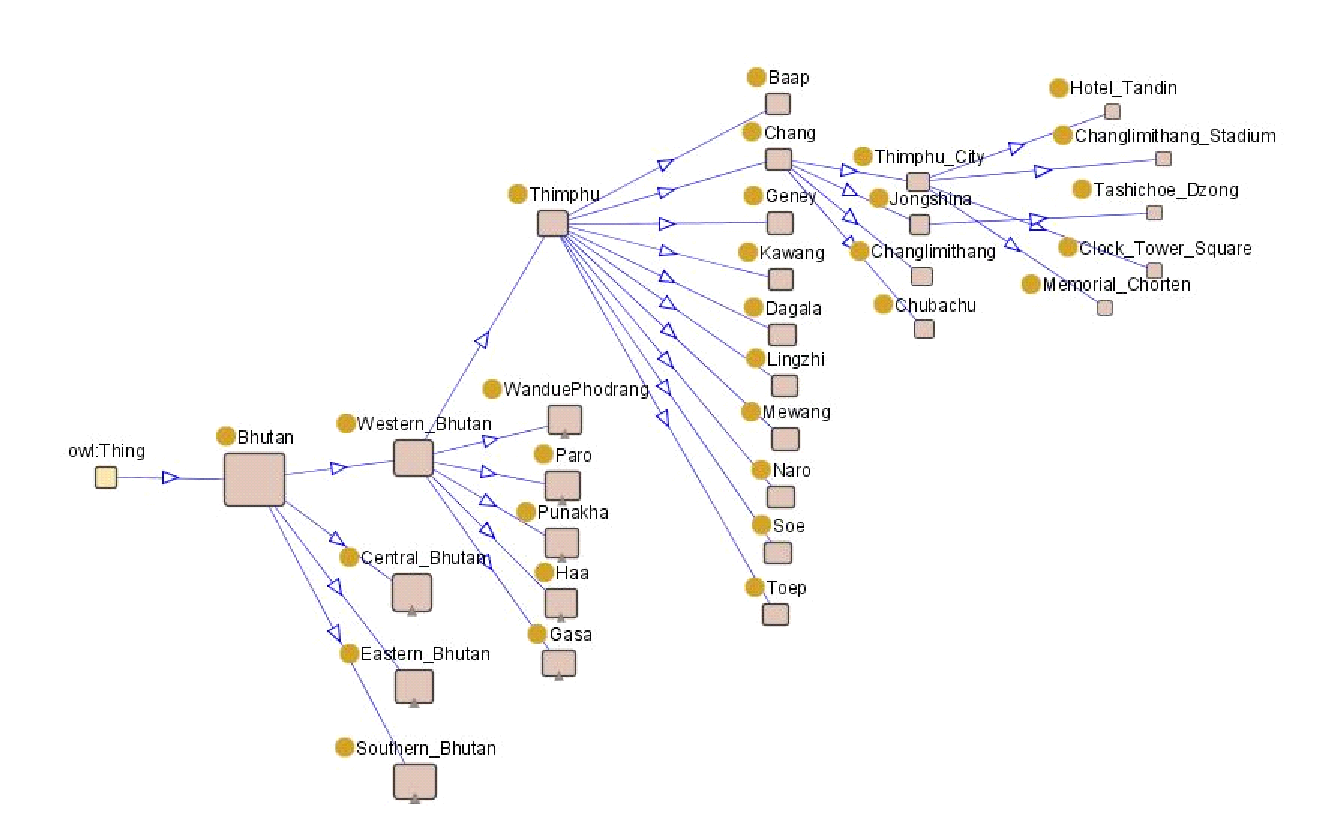
\includegraphics[width=14.8cm, height=10cm]{Bhutan}
\caption {Excerpt of the partonomy of Bhutan}\label{fig:Fig5.3}
\end{center}
\end{figure}

 \textbf{Ground Facts}
\begin{small}
\singlespacing
\begin{verbatim}
 %region(?Province, ?Region)

  region(Thimphu, Western).
  region(Bumthang, Central).
  region(Tashiyangtse, Eastern).
  region(Samtse, Southern).

 %city(?CityC, ?BlockB, ?ProvinceP, ?CountryC, ?AttractionX:Attractions).
 
  city(Thimphu_city,Upper_Thimphu,Thimphu,Bhutan,Tashichoe_Dzong:Fortress).
  town(Paro_town,  Paro_Bazar, Paro, Bhutan, Museum:National_museum).
  village(Shab, Shaba, Paro, Bhutan, Chu_Dzong:Fortress).
  place(Drugedingkha, Shari, Paro, Bhutan, Park:National_park).
\end{verbatim}
\end{small}
\doublespacing

\hspace{0.3in}The ground fact representation of the regions of provinces are constructed by pairing the name of a region and its corresponding province as two arguments of a binary relation. Similarly, attractions are described at the level of subblocks and are used as arguments of one of the five predicates of city, town, village, or place relation. The first ground fact shown above represents the attraction ``Tashichoe\_Dzong" of type fortress is located in the city ``Thimphu\_city", in the block ``Upper\_Thimphu", in the province ``Thimphu", in the Country ``Bhutan". The inference rules that will operate on the above ground facts are implemented as follows:
\\
\begin{small}
    \textbf{KB}
\end{small}

\begin{small}
\singlespacing
\begin{verbatim}
 %An Attraction is in a country if it is in a province of a region 
 %in that country

  country(?Country, ?Attraction:Attractions):- 
    province(?Province, ?Region, ?Country, ?Attraction: Attractions).
  
 %An Attraction is in the province of a region if it is in a block that 
 %is located in province of the same region.
 
  province(?Province, ?Region, ?Country, ?Attraction:Attractions):- 
    block(?Block, ?Province, ?Country, ?Attraction:Attractions),
    region(?Province, ?Region).				 
										 
 %An Attraction is in the block of a province if it is either in a city, 
 %town, village or a place in this block of the same province.	
									 
  block(?Block, ?Province, ?Country, ?Attraction:Attractions):- 
    city(?City, ?Block, ?Province, ?Country, ?Attraction:Attractions).
  
  block(?Block, ?Province, ?Country, ?Attraction: Attractions):- 
    town(?Town, ?Block, ?Province, ?Country, ?Attraction:Attractions).
  
  block(?Block, ?Province, ?Country, ?Attraction:Attractions):- 
    village(?Village, ?Block, ?Province, ?Country, ?Attraction:Attractions).
  
  block(?Block, ?Province, ?Country, ?Attraction:Attractions):- 
    place(?Place, ?Block, ?Province, ?Country, ?Attraction:Attractions).
\end{verbatim}
\end{small}
\begin{small}
\singlespacing
\begin{verbatim}
 %Predicate to get attractions given zero or more constant arguments.

 getAttraction(?Block, ?Province, ?Region, ?Attraction:Attractions):-
   block(?Block, ?Province, ?Country, ?Attraction:Attractions),
   region(?Province, ?Region).
\end{verbatim}
\end{small}
\hspace{0.3in}The above rule can find attraction names located in a specified block, province, or a region. It can also be used to get the name of the block, province, and region of a known attraction. Different modes of queries with different combinations of free variables and constants are shown below. We will assume a user asks for more solutions until none are left.
\\
\begin{small}
    \textbf{Sample Queries}
\end{small}

\begin{small}
\singlespacing
\begin{verbatim}
 %QUERY: getAttraction(?Block, ?Province, ?Region, ?A:Attractions)
 %Solution: It will return all the attractions in the KB since it is an open 
            query (all the arguments are free variables).

 %QUERY: getAttraction(?Block, Paro, ?Region, ?A:Attractions)
 %Solution: It will return all the attractions in the province "Paro"

 %QUERY: getAttraction(?Block, ?Province, Western, ?A:Attractions)
 %Solution: It will return all the attractions in the "Western" Bhutan

 %QUERY: getAttraction(Thimphu_city, ?Province, ?Region, ?A:Attractions)
 %Solution: It will return all the attractions located in the block 
            "Thimphu_city"

 %QUERY: getAttraction(?Block, Paro, ?Region, Memorial_Chorten:Attractions)
 %Solution: It will return the Block of the attraction "Memorial_Chorten:
            Attractions in Paro"
\end{verbatim}
\end{small}

\hspace{0.3in}An attraction's full address can be computed from the facts. This approach is called domain-specific because the predicate names are related to the subparts of the region. The relation names such as city, town, village, or place can be defined as types in our RDFS type definition and used as types to the subblock argument. This extension of enriching partOf with an RDFS type taxonomy is discussed in the next section.

\subsubsection{Enriched Partonomy Rule with Type Definition}
\doublespacing
\hspace{0.3in}We now present an enhanced approach to build the partonomy of a country using chained binary facts. The partonomic differentiation is thus shown as a hierarchy from the highest level of the partonomy (country) to its lowest unit (subblock). Attractions, event locations, and accommodations are located in these subblocks. Every argument in the facts is extended by a type. This adds more knowledge to the arguments. It also shows a clear interrelation between a taxonomy and a partonomy. The main advantage of having this richer representation of knowledge is that it makes our task easier at the rule-implemenation level. We will discuss a good example of this advantage after representating the ground facts. The ground facts shown below are an excerpt from our Bhutan KB; refer to Appendix C to view the complete KB.

\begin{small}
    \textbf{Ground Facts}
\end{small}

\begin{small}
\singlespacing
\begin{verbatim}
 % siteOf(?Attraction:Attractions, ?Subblock:Subblock).
 
  siteOf(Ura_Lhakhang:Temple, Ura_Village:Village).
  siteOf(Bumthang_Dzong:Fortress, Chamkhar:Town).

 %partOfBlock(?Subblock:Subblock, ?Block:Block).

   partOfBlock(Buli:Village, Chhoekhor:Block).
   partOfBlock(Tharpaling:Village, Chhoekhor:Block).
   partOfBlock(Prakar:Village, Chhoekhor:Block).
   partOfBlock(Nimalung:Village, Chhoekhor:Block).
   partOfBlock(Domkhar:Village, Chhoekhor:Block).
   partOfBlock(Chamkhar:Town, Chhoekhor:Block).
   partOfBlock(Tangbi:Village, Chhoekhor:Block).
   partOfBlock{Ura_Village:Village, Ura:Block).

 %partOfProvince(?Block:Block, ?Province:Province).

   partOfProvince(Chhoekhor:Block, Bumthang:Province).
   partOfProvince(Chumme:Block, Bumthang:Province).
   partOfProvince(Tang:Block, Bumthang:Province).
   partOfProvince(Ura:Block, Bumthang:Province).

 %partOfRegion(?Province:Province, ?Region:Region).
 
   partOfRegion(Bumthang:Province, Central:Region).

 %partOfCountry(?Region:Region, ?Country:Country).

   partOfCountry(Central:Region, Bhutan:Country).
\end{verbatim}
\end{small}

\hspace{0.3in}The main advantage of this representation of partonomy facts over the first representation is that it avoids redundant information, and it demonstrates chaining through the binary facts. This definition of our partonomy is then used for various information retrieval tasks in a systematic manner. A simple application  of the partOf hierarchy is the ``getFullAddress" rule shown below. It is used to compute the full address of any attraction in the KB.
\\
\begin{small}
    \textbf{KB}
\end{small}

\begin{small}
\singlespacing
\begin{verbatim}
 getFullAddress(?Location, [?Subblock,?Block,?Province,?Region,?Country]):-
   siteOf(?Location, ?Subblock),
   partOfBlock(?Subblock, ?Block),
   partOfProvince(?Block, ?Province),
   partOfRegion(?Province, ?Region),
   partOfCountry(?Region, ?Country).  
\end{verbatim}
\end{small} 

\begin{small}
    \textbf{Sample Query}
\end{small}
\begin{small}
\singlespacing
\begin{verbatim}
 getFullAddress(Ta_Dzong:National_museum, ?Address)
\end{verbatim}
\end{small} 
\begin{small}
    \textbf{OO jDREW TD Result}
\end{small}
\begin{small}
\singlespacing
\begin{verbatim}
  ?Address=	[Hungrel:Village, 
             Hungrel:Block, 
             Paro:Province, 
             Western:Region, 
             Bhutan:Country]
\end{verbatim}
\end{small}

\hspace{0.3in}The result shown above is an example that demonstrates how the type definition avoids information ambiguity. The address of the museum has the same name for its subblock and block. In Bhutan, it is often the case that the main subblock of a block has the same name as its block. The two kinds of inferences are distinguished by the type definition. We have further extended this work to provide a more precise addressing scheme by including the GPS coordinates of any given locations. We implementated rules that employ facts about the GPS locations. Examples using fictitious data are shown below:
\\
\begin{small}
    \textbf{Sample GPS Facts}
\end{small}

\begin{small}
\singlespacing
\begin{verbatim}
 address(Bumthang_Dzong:Fortress, 
         Loc[latitude->Detail[degree->48:Real; minute->0:Real];
             longitude->Detail[degree->66:Real; minute->40:Real]]).

 address(Zorig_Chusum:Crafts_show, 
         Loc[latitude->Detail[degree->51:Real; minute->6:Real];
             longitude->Detail[degree->114:Real; minute->1:Real]]).

 address(Ugyen_Chholing_Museum:Local_museum, 
         Loc[latitude->Detail[degree->49:Real; minute->11:Real];
             longitude->Detail[degree->123:Real; minute->10:Real]]).
\end{verbatim}
\end{small}

\hspace{0.3in}From such centralized stored facts concerning the longitude and latitude of attraction sites, we can apply the rules ``getLatiLoc" and ``getLongiLoc" to get the latitude and longitude data points, which will be later used for the computation 
of the actual latitude and longitude of a location by the ``getLatitude" and ``getLongitude" relations, respectively.

\begin{small}
\singlespacing
\begin{verbatim}
 getLatiLoc(?Location, ?Degree, ?Minute) :-
   address(?Location, 
           Loc[latitude->Detail[degree->?Degree; minute->?Minute]!?]).

 getLongiLoc(?Location, ?Degree, ?Minute) :-
   address(?Location, 
           Loc[longitude->Detail[degree->?Degree; minute->?Minute]!?]).
 
 %Computes longitude and latitude of a location

  getLatitude(?Location, ?Latitude) :-
    getLatiLoc(?Location, ?Degree, ?Minute),
    divide(?Tmp1, ?Minute, 60:Real),
    add(?Tmp2, ?Degree, ?Tmp1),
    multiply(?Latitude, ?Tmp2, 100:Real).

  getLongitude(?Location, ?Longitude) :-
    getLongiLoc(?Location, ?Degree, ?Minute),
    divide(?Tmp1, ?Minute, 60:Real),
    add(?Tmp2, ?Degree, ?Tmp1),
    multiply(?Longitude, ?Tmp2, 100:Real).
\end{verbatim}
\end{small}

\hspace{0.3in}Considering the GPS points, the enhanced version of the ``getFullAddress" relation is shown next, followed by a sample query and the corresponding result generated in OO jDREW TD.
\\
\begin{small}
    \textbf{Sample KB}
\end{small}

\begin{small}
\singlespacing
\begin{verbatim}
 getFullAddress(?Location, [?Subblock, ?Block, ?Province, ?Region, ?Country, 
                ?Latitude, ?Longitude]):-
   getLatitude(?Location, ?Latitude),
   getLongitude(?Location, ?Longitude),
   siteOf(?Location, ?Subblock),
   partOfBlock(?Subblock, ?Block),
   partOfProvince(?Block, ?Province),
   partOfRegion(?Province, ?Region),
   partOfCountry(?Region, ?Country).
\end{verbatim}
\end{small}

\begin{small}
    \textbf{Sample Query}
\end{small}
\begin{small}
\singlespacing
\begin{verbatim}
 getFullAddress(Bumthang_Dzong:Fortress, ?Address)
\end{verbatim}
\end{small}

\begin{small}
    \textbf{OO jDREW TD Result}
\end{small}
\begin{small}
\singlespacing
\begin{verbatim}
 ?Address=
   [4800.0:Real,
    6666.666666666667:Real,
    Chamkhar:Town,
    Chhoekhor:Block,
    Bumthang:Province,
    Central:Region,
    Bhutan:Country]
\end{verbatim}
\end{small}

\hspace{0.3in} The taxonomy-enriched partonomy rules allow us to search attractions at any subpart of a country. In order to provide an easy search of attractions and flexibility in the search domain to our users, we have implemented five different modes of ``getAttraction", each dealing with a specific sublevel of a country. The recursive ``getAttraction" predicate shown below allows attraction search at any specified subpart of a country.
\pagebreak

\begin{small}
    \textbf{KB}
\end{small}

\begin{small}
\singlespacing
\begin{verbatim}
 %-----at a subblock level---------------------------------------------%

 getAttraction(?Attraction:Attractions, ?Subblock:Subblock):-
   siteOf(?Attraction:Attractions, ?Subblock:Subblock).
 
 %----at a block level-------------------------------------------------%

 getAttraction(?Attraction:Attractions, ?Block:Block):-
   partOfBlock(?Attraction:Attractions, ?Block:Block).
  
 getAttraction(?Attraction:Attractions, ?Block:Block):-
   partOfBlock(?Subblock:Subblock, ?Block:Block),
   getAttraction(?Attraction:Attractions, ?Subblock:Subblock).

 %-----at a province level---------------------------------------------%

 getAttraction(?Attraction:Attractions, ?Province:Province):-
   partOfProvince(?Attraction:Attractions, ?Province:Province).
  
 getAttraction(?Attraction:Attractions, ?Province:Province):-
   partOfProvince(?Block:Block, ?Province:Province),
   getAttraction(?Attraction:Attractions, ?Block:Block).

 %-----at a region  level----------------------------------------------%

 getAttraction(?Attraction:Attractions, ?Region:Region):-
   partOfRegion(?Attraction:Attractions, ?Region:Region).
    
 getAttraction(?Attraction:Attractions, ?Region:Region):-
   partOfRegion(?Province:Province, ?Region:Region),
   getAttraction(?Attraction:Attractions, ?Province:Province).
  
 %----at a country level-----------------------------------------------%

 getAttraction(?Attraction:Attractions, ?Country:Country):-
   partOfCountry(?Attraction:Attractions, ?Country:Country).

 getAttraction(?Attraction:Attractions, ?Country:Country):-
   partOfCountry(?Region:Region, ?Country:Country),
   getAttraction(?Attraction:Attractions, ?Region:Region).
\end{verbatim}
\end{small}
 
\hspace{0.3in}By querying the above rule set, we can find names of attractions at any level of the partonomy, computed one at a time. A remark on the binary ``getAttraction" relation is that it takes care of facts that will not necessarily be at the lowest possible level in the hierarchical partOf definition of a country. For example, an attraction can be directly placed under any subpart of a country. This gives flexibility to knowledge designers, as it is not always possible to know the complete hierarchy levels for some entity locations. For example, the attraction ``Niagra\_Fall" can be directly placed as a partOf Canada (rather than ``Ontario"), and yet the system can find the correct solution.

\hspace{0.3in} Sample search queries and the corresponding results as run in OO jDREW TD for the binary ``getAttraction" relation are shown below:\\
\begin{small}
    \textbf{Sample Queries}
\end{small}

\begin{small}
\singlespacing
\begin{verbatim}
 %To get all the attractions located in the country Bhutan
  getAttraction(?Attraction:Attractions, Bhutan:Country)
 
 %To get all the attractions located in the Western region of Bhutan
  getAttraction(?Attraction:Attractions, Western:Region)
 
 %To get all the attractions located in the province Bumthang
  getAttraction(?Attraction:Attractions, Bumthang:Province)
 
 %To get all the attractions located in the block Chhoekhor
  getAttraction(?Attraction:Attractions, Chhoekhor:Block)
   
 %To get all the attractions located in the subblock Chamkhar of type town
  getAttraction(?Attraction:Attractions, Chamkhar:Town)
 \end{verbatim}
\end{small}

\hspace{0.3in} The solution for the last query ``getAttraction" at the subblock (lowest subdivision of a country) ``Chamkhar",   is shown below. Each of the following attractions are result bindings given one result at a time.
\\
\begin{small}
    \textbf{OO jDREW TD Result}
\end{small}

\begin{small}
\singlespacing
\begin{verbatim}
 ?Attraction= Bumthang_Dzong:Fortress
 ?Attraction= Zugney:Textiles
 ?Attraction=	Ugyen_Chholing_Museum:Local_museum
 ?Attraction= Petseling_Gompa:Temple
\end{verbatim}
\end{small}

\hspace{0.3in} The search results of the ``getAttraction" query can be enriched by retrieving more knowledge from the FOAF-like profiles of each attraction in our KB. In order to provide detailed information about the attraction and its location, we integrated the getFullAddress predicate with getAttraction. The second argument, ``?AttractionDetails", in the query shown after the rule gets bound to the attraction details as shown in the result.
\\
\begin{small}
    \textbf{KB}
\end{small}

\begin{small}
\singlespacing
\begin{verbatim}
 getAttractionDetails(address->[?Subblock,?Block,?Province,?Region,?Country];
                      [Name->?Name; 
                       WebLink->?Url; 
                       Address->[?Subblock, 
                                 ?Block,
                                 ?Province, 
                                 ?Region, 
                                 ?Country];
                       Description->?Description;    
                       RelatedTo->?RelatedTo]):-
    attraction(?Name^hs.url->?Url; 
                     hs.description->?Description; 
                     et.open->?OpenHours;
                     et.theme->?Theme; 
                     et.subblock->?Subblock; 
                     et.province->?Province;  
                     hs.relatedTo->?RelatedTo!?),
    getFullAddress(?Name, [?Subblock,?Block,?Province,?Region,?Country]).
\end{verbatim}
\end{small} 
\begin{small}
    \textbf{Sample query}
\end{small}
\begin{small}
\singlespacing
\begin{verbatim}
 getAttractionDetails(address->[?Subblock, 
                                Hungrel:Block, 
                                ?Province, 
                                ?Region, 
                                ?Country];
                      ?AttractionDetails)
\end{verbatim}
\end{small} 
\begin{small}
    \textbf{OO jDREW TD Result}
\end{small}
\begin{small}
\singlespacing
\begin{verbatim}
 ?AttractionDetails=
   [Name->Ta_Dzong:National_museum;
    WebLink->"www.nationalmuseum.gov.bt/"; 
    Description->"It is the biggest and the oldest museum in Bhutan"; 
    Address->[Goepay:Village, 
              Hungrel:Block, 
              Paro:Province, 
              Western:Region, 
              Bhutan:Country]; 
              RelatedTo->Tashichoe_Dzong:Fortress]
\end{verbatim}
\end{small} 

\hspace{0.3in} This ``getAttraction" predicate can be generalized to a ``getEntity" predicate, which will return the required information for a specified entity. A recursive ``getAttractionList" predicate, which accumulates a number of `N' attractions at a user-specified location is shown below.
\\
\begin{small}
   \textbf{KB}
\end{small}

\begin{small}
\singlespacing
\begin{verbatim}
 %to get a number of N attractions at any level of the partonomy.
 
 getAttractionList(location->?location;
                   visited->?Visited; 
                   attractionList->[]; num->0). 
  
 getAttractionList(location->?location;
                   visited->?Visited; 
                   attractionList->[?Attraction|?Rest];  
                   num->?N:Integer):-
   greaterThan(?N:Integer, 0:Integer),
   getAttraction(?Attraction, ?location),
   notMember(?Attraction, ?Visited),
   subtract(?Numtleft, ?N:Integer,  1:Integer),
   getAttractionList(location->?location;   
                     visited->[?Attraction|?Visited]; 
                     attractionList->?Rest;  
                     num->?Numtleft).
\end{verbatim}
\end{small} 
\begin{small}
    \textbf{Sample query}
\end{small}
\begin{small}
\singlespacing
\begin{verbatim}
 getAttractionList(location->Chamkhar:Town;
                   visited->[]; 
                   attractionList->?AttractionList; 
                   num->3:Integer) 
\end{verbatim}
\end{small} 
\begin{small}
    \textbf{OO jDREW TD Result}
\end{small}
\begin{small}
\singlespacing
\begin{verbatim}
 ?AttractionList=
 	 [Bumthang_Dzong:Fortress, 
 	  Zugney:Textiles, 
 	  Ugyen_Chholing_Museum:Local_museum]
\end{verbatim}
\end{small} 

\subsubsection{General Partonomy Rule}

\hspace{0.3in} Partonomy rules, however, can be made more general, so that they are less restricted by the domain of interest. A generic definition of the ``partOf" relation can be used for describing the entire partonomy of any domain. The transitive closure of the binary ``partOf" relation allows us to do any depth of chaining, from a given superpart of the hierarchy to the lowest subpartOf property. An example of such a derivation of facts is shown below. In this design, we need to describe every subpart relation by the same binary predicate name ``partOf". We can define partOfTrans for chaining through pairs of partOf ground facts.
\\
\begin{small}
    \textbf{KB}
\end{small}

\begin{small}
\singlespacing
\begin{verbatim}
 partOfTrans(?X, ?Y):- 
   partOf(?X, ?Y).

 partOfTrans(?X, ?Z):-
   partOf(?X, ?Y),
   partOfTrans(?Y, ?Z).
\end{verbatim}
\end{small}

\hspace{0.3in}Assuming, our facts are all defined with one common generic name, ``partOf", the partOfTrans predicate can explore the entire partonomy as well as check the subparts of each relation by instantiating one of the two arguments. Similar to the first approach, we can generate new variable bindings by using different combinations of constants and free variables in the query. Some facts, a sample query, and the variable bindings in the output generated by OO jDREW TD are shown below.
\\
\begin{small}
    \textbf{Ground Facts}
\end{small}

\begin{small}
\singlespacing
\begin{verbatim}
 %partOf(?SubPart, ?SuperPart).
 
  partOf(Chamkhar:Town, Chhoekhor:Block).
  partOf(Chhoekhor:Block, Bumthang:Province).
  partOf(Bumthang:Province, Central:Region).
  partOf(Central:Region, Bhutan:Country).
\end{verbatim}
\end{small}

\begin{small}
\textbf{Sample Query}
\end{small}
\begin{small}
\singlespacing
\begin{verbatim}
partOfTrans(?SubPart, ?SuperPart)
\end{verbatim}
\end{small}

\begin{small}
    \textbf{OO jDREW TD Result}
\end{small}
\begin{small}
\singlespacing
\begin{verbatim}
 First Solution:
 ?SubPart=	Chamkhar:Town
 ?SuperPart=	Chhoekhor:Block
 
 Next Solution:
 ?SubPart=	Chhoekhor:Block
 ?SuperPart=	Bumthang:Province
 
 Next Solution:
 ?SubPart=	Bumthang:Province
 ?SuperPart=	Central:Region
 
 Next Solution: 
 ?SubPart=	Central:Region
 ?SuperPart=	Bhutan:Country
 
 Next Solution:
 ?SubPart=	Chamkhar:Town
 ?SuperPart=	Bumthang:Province
 
 Next Solution:
 ?SubPart=	Chhoekhor:Block
 ?SuperPart=	Central:Region
 
 Next Solution:
 ?SubPart=	Bumthang:Province
 ?SuperPart=	Bhutan:Country
 
 Next Solution:
 ?SubPart=	Chamkhar:Town
 ?SuperPart=	Central:Region

 Next Solution:
 ?SubPart=	Chhoekhor:Block
 ?SuperPart=	Bhutan:Country 

 Last Solution:
 ?SubPart=	Chamkhar:Town
 ?SuperPart=	Bhutan:Country
 \end{verbatim}
\end{small} 

\hspace{0.3in}This query will bind its variables to every pair of partOf instances in the KB. Using the same facts, we can derive more specific facts by instantiating one of the arguments in the query:

\begin{small}
\singlespacing
\begin{verbatim}
 partOfTrans(?SubPart, Chhoekhor:Block)

 Variable binding:
  ?SubPart=	 Chamkhar:Town
\end{verbatim}
\end{small}

\hspace{0.3in}This query has its second argument instantiated to the constant ``Chhoekhor:Block", and the system returns all variable bindings of ``?SubPart" that are parts of the block ``Chhoekhor:Block". Similarly, we can find parts of any province, region, or the country. We can also perform all the domain-specific queries that were shown in our first approach such as get attraction address. Like in our type-enriched domain-specific partonomy, every part has either exactly one or no superpart etc, down to the leaves level. The highest level of our hierarchy, ``country", has no superpart and the lower sublevels have exactly one unique superpart. 

\hspace{0.3in}However, domain-specific partonomy rules are used in this thesis, so as to speed up the execution time by narrowing down the search space for each specific rule set. Please refer to Appendix C to view the complete partonomy of Bhutan.

\subsection{Distance Computation}

\hspace{0.3in}Taking into account the importance of measuring distance for any kind of travel planning, we considered the aspect of distance computation as one of the two primary auxiliary rule sets.

\hspace{0.3in}The implementation of the distance computation KB has been first tested solely in the OO jDREW Top-down Backward Reasoner. From the various architectural features of OO jDREW described in Section 3.3, we found the TD FindAll Solutions architecture the most suitable for the precomputation of routes and distance times.

\subsubsection{Precomputation of All Routes}

\hspace{0.3in}The transitive closure database consists of ternary ``distanceTime" ground facts, which represent the distances between adjacent nodes measured in  bus hours. % for four different modes of transportation.
The distance computation rule subsystem has been tested for sample graphs as shown in Figure 5.4. In this example, we have only considered a single mode of transportation. However, in our complete KB (cf. Appendix C), we considered four modes of transportation, namely bus, taxicab, bicycle, and hiking. The bus distance time, measured in hours, for each connected pair of nodes in Figure 5.4 is represented as shown below: 

\begin{figure}
\begin{center}
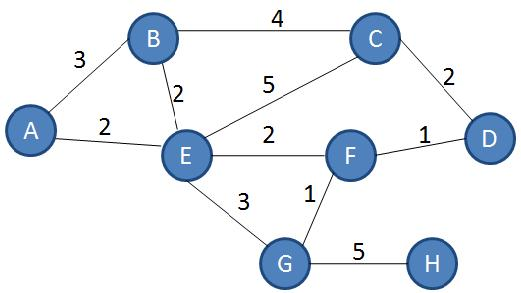
\includegraphics[width=13cm, height=9cm]{graph1}
\caption {Connected graph for distance computation}
\label{fig:Fig5.2}
\end{center}
\end{figure}

\begin{small}
\textbf{Ground facts}
\end{small}

\begin{small}
\singlespacing
\begin{verbatim}
%distanceTime(startPoint->?Province1; endPoint->?Province2; bus->?Bus: Real)
 
 distanceTime(startPoint->A; endPoint->B; bus->3:Real).
 distanceTime(startPoint->A; endPoint->E; bus->2:Real). 
 distanceTime(startPoint->B; endPoint->C; bus->4:Real).
 distanceTime(startPoint->B; endPoint->E; bus->2:Real).
 distanceTime(startPoint->E; endPoint->F; bus->2:Real). 
 distanceTime(startPoint->C; endPoint->D; bus->2:Real).
 distanceTime(startPoint->C; endPoint->E; bus->5:Real). 
 distanceTime(startPoint->D; endPoint->F; bus->1:Real). 	
 distanceTime(startPoint->E; endPoint->G; bus->3:Real).
 distanceTime(startPoint->F; endPoint->G; bus->1:Real). 	
 distanceTime(startPoint->G; endPoint->I; bus->5:Real). 
	
\end{verbatim}
\end{small}

We obtain the bidirectional routes between locations by applying the symmetric rule on the transitive closure ground facts as shown below:

\pagebreak 
\begin{small}
\textbf{KB}
\end{small}

\begin{small}
\singlespacing
\begin{verbatim}
 distanceTimeSymmetric(startPoint->?Province1; 
                       endPoint->?Province2; 
                       bus->?Bus:Real):-
   distanceTime(startPoint->?Province1; 
                endPoint->?Province2; 
                bus->?Bus:Real).

 distanceTimeSymmetric(startPoint->?Province1; 
                       endPoint->?Province2; 
                       bus->?Bus:Real):-
   distanceTime(startPoint->?Province2; 
                endPoint->?Province1; 
                bus->?Bus:Real). 
\end{verbatim}
\end{small}

\hspace{0.3in}In order to compute the route and the distance time measured in hours between any two nodes in the graph, we implemented the recursive ``distanceTimeRoute"  predicate. The ``notMember" predicate is used to avoid de-touring in the routes. The  ``dTR" predicate is the interface predicate, which in turn enforces the ``distanceTimeRoute" workhorse predicate to compute the route and bus hours between any two nodes. For efficiency reason, all routes between every pair of nodes are precomputed by using the Top-Down FindAll Solutions architecture.
\\
\begin{small}
\textbf{KB}
\end{small}

\begin{small}
\singlespacing
\begin{verbatim}
 %Interface predicate to enforce the distanceTimeRoute main predicate
 
  dTR(startPoint->?Province1; 
      endPoint->?Province2; 
      route->?Route; 
      totalTime->?TotalBusHours):-
    distanceTimeRoute(startPoint->?Province1; 
                      endPoint->?Province2; 
                      [], 
                      0:Real; 
                      route->?Rest; 
                      totalTime->?TotalBusHours).

 %Workhorse predicate to compute the routes and bushours for any two provinces
  
 distanceTimeRoute(startPoint->?Province; 
                   endPoint->?Province; 
                   ?Visited, 
                   ?AccumulateTime:Real; 
                   route->[?Province];  
                   totalTime->?AccumulateTime:Real).

 distanceTimeRoute(startPoint->?Province1; 
                   endPoint->?ProvinceX; 
                   ?Visited, 
                   ?AccumulateTime:Real; 
                   route->[?Province1|?Rest];  
                   totalTime->?TotalBusHours:Real):-  
  distanceTimeSymmetric(?Province1, ?Province2; bus->?Bus!?),
  notMember(?Province2, ?Visited),
  add(?NewBus, ?Bus, ?AccumulateTime:Real),
  distanceTimeRoute(startPoint->?Province2; 
                    endPoint->?ProvinceX; 
                    [?Province1,?Province2|?Visited], 
                    ?NewBus; 
                    route->?Rest; 
                    totalTime->?TotalBusHours:Real).
  
 %Query: dTR(startPoint->?Province1; endPoint->?Province2; 
             route->?Route; totalTime->?TotalBusHours)               
\end{verbatim}
\end{small}

\hspace{0.3in}The dTR predicate was executed in the Top-Down FindAll Solutions with the open query (i.e., free variables for all slot fillers) shown above. Top-Down FindAll Solutions performs an iterative deepening of every connected nodes in the graph, which generates a new set of ``dTR" facts. Each dTR fact represents a route and corresponding bus hours between a pair of nodes. For example, the newly generated dTR facts for the start point ``A" to the end point ``D" are as shown below:
 
\begin{small}
\textbf{OO jDREW FindAll Solutions Result}
\end{small}

\begin{small}
\singlespacing
\begin{verbatim}
%Query:dTR(startPoint->A;endPoint->D;route->?Route;totalTime->?TotalBusHours)
  
%Generated Facts:
 dTR(startPoint->A;endPoint->D;route->[A,B,C,D];totalTime->9.0:Real).
 dTR(startPoint->A;endPoint->D; route->[A,E,F,D];totalTime->5.0:Real).
 dTR(startPoint->A;endPoint->D;route->[A,E,C,D];totalTime->9.0:Real).
 dTR(startPoint->A;endPoint->D;route->[A,B,E,F,D];totalTime->8.0:Real).
 dTR(startPoint->A;endPoint->D;route->[A,B,E,C,D];totalTime->12.0:Real).
 dTR(startPoint->A;endPoint->D;route->[A,E,G,F,D];totalTime->7.0:Real).
 dTR(startPoint->A;endPoint->D;route->[A,E,B,C,D];totalTime->10.0:Real).
 dTR(startPoint->A;endPoint->D;route->[A,B,C,E,F,D];totalTime->15.0:Real).
 dTR(startPoint->A;endPoint->D;route->[A,B,E,G,F,D];totalTime->10.0:Real).
 dTR(startPoint->A;endPoint->D;route->[A,B,C,E,G,F,D];totalTime->17.0:Real).
 routeCount(startPoint->A;endPoint->D;totalCount->10:Integer).
\end{verbatim}
\end{small}

\hspace{0.3in} There are 10 different routes connecting the start point ``A" to the end point ``D". The total bus hours for all the routes are given by the slot name ``totalTime". These generated dTR facts form the basis of route planning operations. For example, they can be used to answer simple queries such as ``find all possible routes and their distance times" between any two provinces. Next, we applied some optimization rules on the dTR facts to solve queries such as to find the shortest path from the set of all possible routes. Our approach to solve this problem is described in the next section.

\subsubsection{Shortest Path Computation}

\hspace{0.3in}The transitive closure database executed in the Top-down FindAll Solutions Architecture generates all routes between two specified locations and a count of generated routes. The ``dTRShortest" interface predicate calls the recursive predicate ``dTRList" to compute the shortest route with the shortest bus hours. For example, the shortest route for start point ``A" to end point ``D" is 5 hours with route-$>$[A, E, F, D]. 

\hspace{0.3in}Since we have precomputed all routes and bus hours, the OO jDREW reasoning engine can compute solutions to any queries on top of these quickly. %This approach also allows us to generate the optimal shortest path solution. The total time taken to generate routes between every pair of nodes of the graph in Figure 5.3 is ***
%@@@OO jDREW time measure and efficiency of  this method.%
\\
\begin{small}
\textbf{KB}
\end{small}

\begin{small}
\singlespacing
\begin{verbatim}
%Interface predicate that enforces the workhorse predicate "dTRList"
 dTRShortest(startPoint->?Province1;  
             endPoint->?Province2; 
             routeList->?Routes; 
             shortest->?ShortestRoute):-
   routeCount(startPoint->?Province1;
              endPoint->?Province2;
              count->?Count:Integer),
   dTRList(startPoint->?Province1;  
           endPoint->?Province2; 
           route->?Routes;  
           visited->[];   
          %Initializes the current minimum route to a very large bus hours
           currentMinRoute->[R, 10000:Real];  
           min->?ShortestRoute; 
           count->?Count:Integer).

%Workhorse recursive predicate to compute the min routes from all routes 
 dTRList(startPoint->?Province1;  
         endPoint->?Province2;  
         route->[];  
         visited->?Visited;   
         currentMinRoute->?NewMinRoute;  
         min->?NewMinRoute; 
         count->0:Integer).
 
 dTRList(startPoint->?Province1;  
         endPoint->?Province2;  
         route->[[?R1,?T1]|?Rest];  
         visited->?Visited;   
         currentMinRoute->[?RMin, ?TMin];  
         min->?FinalMinRoute; 
         count->?Count:Integer):-
  dTR(startPoint->?Province1; 
      endPoint->?Province2; 
      route->?R1; 
      totalTime->?T1),
  notMemberList(?R1,?Visited),
  minRoute([[?R1, ?T1], [?RMin, ?TMin]], ?NewMinRoute),
  subtract(?newCount, ?Count:Integer,  1:Integer),
  dTRList(startPoint->?Province1;  
          endPoint->?Province2;  
          route->?Rest; 
          visited->[?R1|?Visited];   
          currentMinRoute->?NewMinRoute; 
          min->?FinalMinRoute; 
          count->?newCount:Integer).

%notMemberList predicate to avoid duplicate list within a list of lists:
 notMemberList( ?X, []).
 notMemberList( ?X, [?H]) :- naf(equalList(?X, ?H)).
 notMemberList( ?X,[?H|?T]) :- naf(equalList(?X, ?H)), notMemberList(?X,?T).

%Checks if two ground lists are equal
 equalList(?L, ?L).

%Simplified minRoute since the list doesnot contain more than two elements
 minRoute([[?R1,?A],[?R2,?B]], [?R1, ?A]) :- lessThan(?A ,?B).
 minRoute([[?R1,?A],[?R2,?B]], [?R2, ?B]) :- lessThan(?B ,?A).

%Query: 
 dTRShortest(startPoint->A;  
             endPoint->D; 
             routeList->?Routes; 
             shortest->?ShortestRoute)           
\end{verbatim}
\end{small}

\hspace{0.3in}The workhorse predicate ``dTRShortest" returns the shortest route and its distance time measured in hours.
In order to use the entire optimised solution as precomputed facts that can provide all routes and their distance times, along with the shortest route, we have precomputed the shortest routes between every pair of nodes by partially transcribing the above ``dTRList" predicate in Java %(i.e. list accumulation), 
and applying the ``minRoute" predicate (cf. Appendix C) in Top-Down FindAll Solutions, which returns the new ``dTRShortest" facts for every pair of nodes in the graph. The new set of dTRShortest facts are used as the KB for any route information required for route planning or for distance validation in the main planner's rule system. %The generated dTRShortest facts for Bhutan's road map which connects 24 nodes (i.e. Provinces) are also shown in Appendix C. 
Route computations are usually implemented using imperative programs such as Dijkstra's Algorithm. However, for the purpose of this thesis, we have tried to keep this computation purely declarative as well. Alternatively, we could use any algorithm from existing Java libraries and load its results as precomputed facts into our KB.

\section{Rule Subsystem for eTourPlan Subdomains}

\subsection{Rule System for Route Planning}
\hspace{0.3in} The main function of a route planner is to find a route that meets users' needs such as preferred transportation mode and preferred intermediate provinces for a route. Route planning is considered as a separate subsystem but most of its functionalities are interleaved in the main travel planner. The various options for route planning are discussed in the following subsections.

\subsubsection{Searching Routes Between Provinces} 
\hspace{0.3in} The eTourPlan prototype can function as a search engine to find all alternative routes between any two provinces specified by a user. Users can make a selection of their preferred transportation mode. This search rule subsystem returns all the routes and the distance time measured in hours for each of the routes, along with a recommendation of the shortest route. The subsystem primarily employs the precomputed ``dTRShortest" route and distance time facts to find all possible routes connecting the user-specified start and end province. The advantage of using precomputed facts is the fast retrieval of solutions to the user's query.

In the sample rule shown below, the ``getRouteDetails" rule will unify the two arguments, route and bus hour by looking through the ``dTRShortest" premises in the KB. The sample query shown below asks for all routes that connect the starting province ``Paro", a province in the Western region, to a destination province ``Trashigang", in the Eastern region of Bhutan. The routes can be seen on the road map of Bhutan shown in Figure 5.5. The transportation mode used for the distance time computation here is ``bus".
\\
\begin{small}
    \textbf{KB}
\end{small}

\begin{small}
\singlespacing
\begin{verbatim}          
 getRouteDetails(startPoint->?ProvinceA;  
                 endPoint->?ProvinceB;  
                 ?Routes,  
                 ?ShortestRoute):- 
   dTRShortest(startPoint->?ProvinceA; 
               endPoint->?ProvinceB; 
               routeList->?Routes; 
               shortest->?ShortestRoute).
\end{verbatim}
\end{small}   
  
 \begin{small}
    \textbf{Sample Query}
\end{small}
\begin{small}
\singlespacing
\begin{verbatim}
getRouteDetails(startPoint->Paro:Province;  
                endPoint->Trashigang:Province;  
                ?Routes,
                ?ShortestRoute)
\end{verbatim}
\end{small}   


 \begin{small}
    \textbf{OO jDREW TD Result}
\end{small}
\begin{small}
\singlespacing
\begin{verbatim}
 ?Routes=
 	[[[Paro, Chuzom, Thimphu, Lobesa, WangduePhodrang, Trongsa, 
 	   Bumthang, Mongar, Trashigang], 30.7:Real], 
 	[[Paro, Chuzom, Thimphu, Lobesa, Punakha, WangduePhodrang, 
 	  Trongsa, Bumthang, Mongar, Trashigang], 31.4:Real], 
 	[[Paro, Haa, Chuzom, Thimphu, Lobesa, WangduePhodrang, Trongsa, 
 	  Bumthang, Mongar, Trashigang], 36.2:Real], 
 	[[Paro, Haa, Chuzom, Thimphu, Lobesa, Punakha, WangduePhodrang, 
 	   Trongsa, Bumthang, Mongar, Trashigang], 36.9:Real], 
 	[[Paro, Chuzom, Thimphu, Lobesa, WangduePhodrang, Damphu, Sarpang, 
 	  Gelephu, Zhemgang, Trongsa, Bumthang, Mongar, Trashigang], 50.7:Real], 
 	[[Paro, Chuzom, Thimphu, Lobesa, Punakha, WangduePhodrang, Damphu, Sarpang, 
 	  Gelephu, Zhemgang, Trongsa, Bumthang, Mongar, Trashigang], 51.4:Real], 
 	[[Paro, Haa, Chuzom, Thimphu, Lobesa, WangduePhodrang, Damphu, Sarpang, 
 	  Gelephu, Zhemgang, Trongsa, Bumthang, Mongar, Trashigang], 56.2:Real], 
 	[[Paro, Haa, Chuzom, Thimphu, Lobesa, Punakha, WangduePhodrang, Damphu, 
 	  Sarpang, Gelephu, Zhemgang, Trongsa, Bumthang, Mongar, Trashigang], 
 	  56.9:Real]]
 	  
 ?ShortestRoute=
	 [[Paro, Chuzom, Thimphu, Lobesa, WangduePhodrang, 
     Trongsa, Bumthang, Mongar, Trashigang], 30.7:Real]

\end{verbatim}
\end{small}   
\begin{figure}
\begin{center}
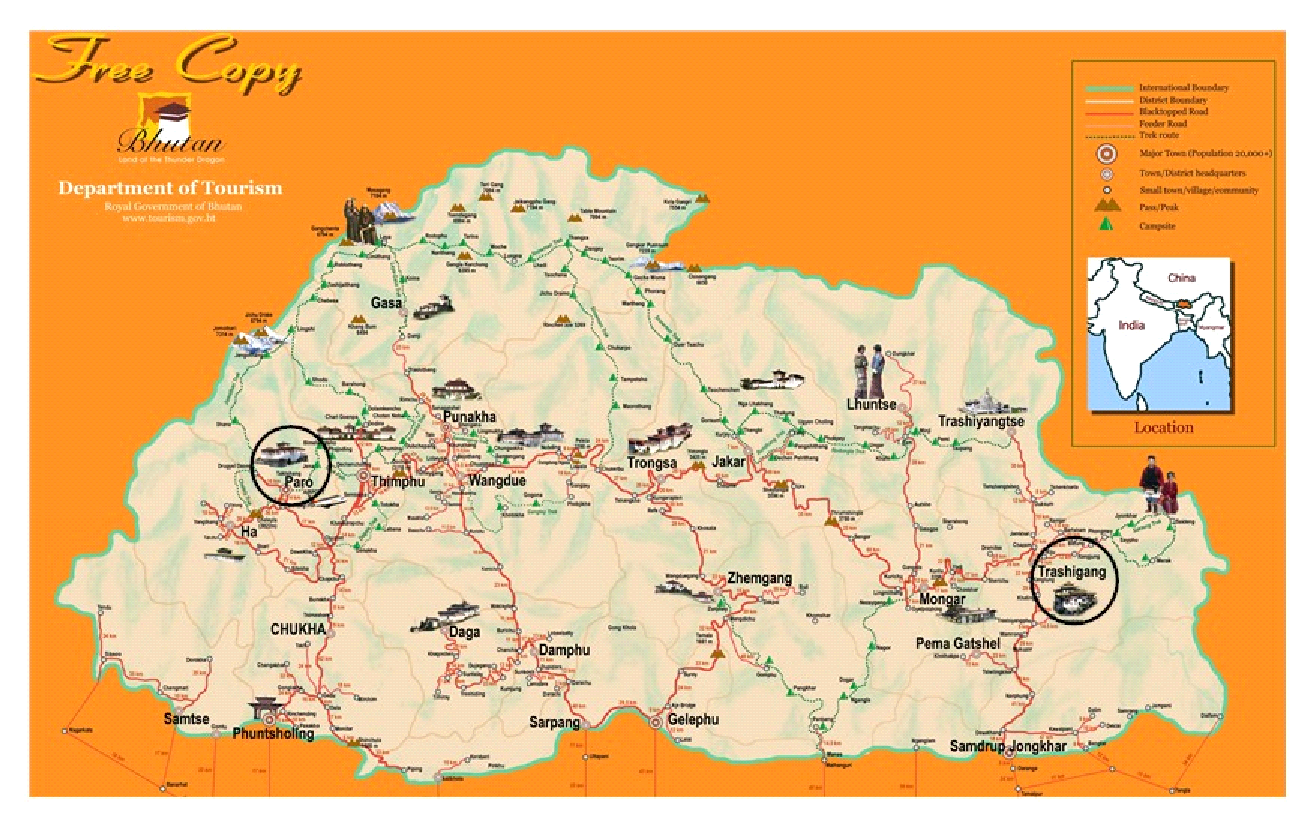
\includegraphics[width=14cm, height=8.5cm]{roadMap}
\caption {Road map of Bhutan (Source:Department of Tourism,Bhutan)}
\label{fig:Fig5.4}
\end{center}
\end{figure} 

The system returns eight alternative routes connecting ``Paro" to ``Trashigang", and the shortest route between these two provinces takes 30.7 hours. It takes only 260 milliseconds to retrieve this route information from the KB. This part of our work can also be useful for other organizations, such as road and transportation service providers.

%\subsubsection{Route planning based on Shortest Distance[i75\%][25w\%]}
%\hspace{0.3in} In order to get the optimal distance in terms of distance hours, we need to pick the shortest route available. The shortest route measured in terms of hours can be retrieved by employing the shortest path auxiliary predicate ``OptDTR" discussed earlier in Section 5.2.1. We can retrieve the shortest route between any two points of location on the road map. The distance computation is done only between provinces in this thesis. However, the current KB can be enhanced to include distance measurement between towns, cities and villages within a province.%


\subsubsection{System Route Planning based on Province Profiles}

Another option offered to our users for route planning is the system's recommendation. We use FOAF-like profiles of provinces described in our KB (cf. Figure 4.1) by chaining through the related provinces to select the next province to visit. Recommendations of locations or touristic provinces are made by referring to the slot filler of the slot name ``hs.relatedTo" in the FOAF-like province profiles in the KB. This slot represents the related neighbouring provinces from a touristic point of view. Therefore, we use this concept to provide recommendations of most related provinces and find a touristic route for our users.

\hspace{0.3in} Users need to specify the number of provinces, a starting province from the list of FOAF-related provinces and an end province, which can be anywhere in the country. The system finds the best recommended route based on FOAF-like profiles, and it also computes the distance time as it moves from the starting province to the next related province. The resulting route is a chain of related touristic provinces. This predicate is used solely for route planning because we do not yet integrate any recommendation of activities or accommodation facilities in this rule subsystem. This route planner is extended to a location-centric recommender of tourist activities (discussed in Section 5.2.4).

\hspace{0.3in}Let us look at the main route planning predicate here. The interface rule ``routePlanner" calls the recursive ``systemRoutePlanner" predicate (cf. Appendix C) and the ``shortestRoute" predicate. The ``shortestRoute" predicate finds the shortest route from the last visited province to a user's specified end point. A sample query, which queries the system to recommend 5 provinces to visit, starting at ``Paro" and ending at ``Gelephu", is shown after representing the route planner rule. The result from our KB is a list of 5 FOAF-related provinces with details of route and distance time for each hop. It also provides the final route to the user's specified end point.
\\
\\
\\
\begin{small}
    \textbf{KB}
\end{small}

\begin{small}
\singlespacing
\begin{verbatim}
 routePlanner(typeOfPlan->SystemRecommend;
              startPoint->?Province1;  
              endPoint->?ProvinceN;  
              routeDetails->[RecommendedRoute->?Route; 
                             TotalTime->?TotalBusHours;  
                             ReturnRoute->?ReturnRoute];
              numofProvinces->?Num:Integer):-
  systemRoutePlanner(startPoint->?Province1; 
                     nextPoint->?Province2; 
                     toRoute->?Route; 
                     starttime->0:Real; 
                     totalTime->?TotalBusHours:Real; 
                     numofProvinces->?Num:Integer ),
  shortestRoute(?Province2, ?ProvinceN, ?ReturnRoute).
\end{verbatim}
\end{small}   
  
 \begin{small}
    \textbf{Sample Query}
\end{small}
\begin{small}
\singlespacing
\begin{verbatim}
routePlanner(typeOfPlan->SystemRecommend;
             startPoint->Paro:Province;  
             endPoint->Gelephu:Province;  
             routeDetails->?RouteDetails;
             numofProvinces->5:Integer)             
\end{verbatim}
\end{small}   

\begin{small}
    \textbf{OO jDREW Result}
\end{small}

\begin{small}
\singlespacing
\begin{verbatim}
 ?RouteDetails=
 	[RecommendedRoute->[[[Paro, Chuzom, Thimphu], 4.5:Real], 
                      [[Thimphu, Lobesa, Punakha], 4.2:Real], 
                      [[Punakha, WangduePhodrang], 0.7:Real], 
                      [[WangduePhodrang, Trongsa], 3.5:Real]];
  ReturnRoute->[[Trongsa,Zhemgang, Gelephu], 8.5:Real]; 
  TotalTime->12.90:Real]
\end{verbatim}
\end{small} 

\subsubsection{Route Planning via User-Preferred Provinces} 

\hspace{0.3in} The system route planner discussed in the previous section has the advantage of finding a complete route guide for users. On the other hand, it has the restriction of providing only for limited preference by users. Therefore, we considered another option for route planning that allows users to include a list of their preferred provinces as intermediate stops between their specified start and end points. The system returns the route and the distance time in bus hours between each of the provinces, along with the total distance time for the entire trip. 

\hspace{0.3in}The interface rule ``routePlanner"  employs the workhorse ``userPrefRoutePlanner" predicate (cf. Appendix C), which includes the list of user-preferred provinces as intermediate stops on the route. The rule is followed by a sample query and its output generated by OO jDREW TD:
\\
\begin{small}
    \textbf{KB}
\end{small}

\begin{small}
\singlespacing
\begin{verbatim}
 %Interface predicate
 routePlanner(typeOfPlan->UserPrefBased;
              startPoint->?Province1;  
              endPoint->?Province2;  
              userPref->?PrefList; 
              routeDetails->[Route->?Route;   
                             TotalTime->?TotalBusHours]):-
   userPrefRoutePlanner(startPoint->?Province1; 
                        endPoint->?Province2; 
                        userPref->?PrefList; 
                        route->?Routes;
                        accumulateTime->0:Real; 
                        totalTime->?TotalBusHours).                  
\end{verbatim}
\end{small} 
\begin{small}
    \textbf{Sample Query}
\end{small}
\begin{small}
\singlespacing
\begin{verbatim}
 routePlanner(typeOfPlan->UserPrefBased;
              startPoint->Paro:Province;  
              endPoint->Paro:Province;  
              userPref->[Thimphu:Province, 
                         Punakha:Province, 
                         Bumthang:Province, 
                         Trashigang:Province]; 
              routeDetails->?RouteDetails)
\end{verbatim}
\end{small}

 \begin{small}
    \textbf{OO jDREW Result}
\end{small}
\begin{small}
\singlespacing
\begin{verbatim}
 ?RouteDetails=
	 [Route->[[[Paro, Chuzom, Thimphu], 4.5:Real], 
            [[Thimphu, Lobesa, Punakha], 4.2:Real], 
            [[Punakha, WangduePhodrang, Trongsa, Bumthang], 8.7:Real], 
            [[Bumthang, Mongar, Trashigang], 14.0:Real], 
             [Trashigang, Mongar, Bumthang, Trongsa, WangduePhodrang, 
						  Lobesa, Thimphu, Chuzom, Paro], 30.7:Real]; 
   TotalTime->62.10:Real]
\end{verbatim}
\end{small}   

\hspace{0.3in}The route planning subsystem returns routes connecting all the provinces in the user's preference list, starting at the specified start point and ending at the specified end point. It also computes the total bus hours for the entire trip. %For an average route planning with two user-preferred provinces in the list, the system takes 11688 milliseconds to generate the results.

\subsection{Rule System for Activity and Accommodation Search}

\hspace{0.3in}``Activity", in the context of our KB, subsumes both the events and attractions subdomains. In this section, we will discuss rules that provide our users with different options to get tourist information from the KB. The parametric search operations that can be performed for any of the tourist entities are explained. 

\subsubsection{Parametric Search for Activity Details}
 
\hspace{0.3in}The activity subdomain of our KB consists of well-structured profiles for activities found in a province. This aspect of our KB contributes to providing detailed search results to our users. The first option offered to users is the ability to find the key information concerning any activity by specifying the activity name. For example, for users who are seeking to learn more about certain festivals or attraction sites, our system can provide all the necessary information from the KB. The main predicate ``getActivityDetails" (cf. Appendix C) provides parametric search of activities (i.e., events and attractions). Users can query this predicate to get the details of a specified activity or to search activities by type or theme in some part of the country. A sample query to get activity details by name and its result are shown below:

\begin{small}
    \textbf{Sample Query}
\end{small}

\begin{small}
\singlespacing
\begin{verbatim}
 getActivityDetails(actName->Paro_Tshechu:Events; ?ActivityDetails!?)
 %Remark: "!?" is used to ignore irrelevant slots in the query.   
\end{verbatim}
\end{small}   
  
 
 \begin{small}
    \textbf{OO jDREW TD Result}
\end{small}
\begin{small}
\singlespacing
\begin{verbatim}
 ?ActivityDetails=
  	[ActName->Paro_Tshechu:Events; 
     Theme->Cultural_Religious_Heritage; 
     EventDates->[StartDate->date[2008:Real, 03:Real, 17:Real]; 
                  EndDate->date[2008:Real, 03:Real, 21:Real]];
     WebLink->" ";
     Description->"Paro Tshechu (Festival) is one of most important 
     festival of Bhutan which starts in spring. The most magnificient 
     thing about it is the unraveling of a large Thanka (Thongdrol)."; 
     Address->[Hungrel:Village, 
               Hungrel:Block, 
               Paro:Province, 
               Western:Region,
               Bhutan:Country];  
     RelatedTo->"Ura_Yakchoe:Annual_festival"]                 
\end{verbatim}
\end{small}

\hspace{0.3in} Activities has two top-level types, attractions and events. Users can provide their preferred type of activity at the top-level or be more specific by specifying a subclass of one of the two main types. For example, a user might want to search only for events of type ``Annual\_festival" or attractions of type ``Historical\_buildings". These type classifications of tourist entities are according to the standards followed by the Harmonise ontology discussed earlier (in Section 2.3). Activities in our KB are categorized into three main themes: Cultural\_Religious\_Heritage, Nature, and Recreation. This categorization is officially used by the Department of Tourism of Bhutan. Our users can perform top-level searches of activities by their preferred theme. Since we have object-centric profiles for each of the activity entities, the system can provide detailed activity information according to the user's specified theme. 
 
\hspace{0.3in}In addition to the above two parameters, users can be more specific about the search area (i.e., Country, Region, Province, Block, Subblock) from the administrative partonomy of a country discussed earlier (in Section 5.1). For example, users can search for activities from a very specific search space of subblocks or broaden the search space, such as searching in a province or within a country as a whole. 

\hspace{0.3in}Therefore, the system provides flexibility of search space for users' queries. The complete predicate definition is shown in Appendix C. A sample query shown below queries for activities of type ``Annual\_festival", in the block ``Chhoekhor:Block". The system will return all the activities that meet the user's specified activity type in a given search area. The first solution to this query is shown below (further solutions would include detailed information of rest of the activities of type ``Annual\_festival" found in the block Chhoekhor).
\\
\begin{small}
    \textbf{Sample Query}
\end{small}

\begin{small}
\singlespacing
\begin{verbatim}
 getActivityDetails(actName->?Name:Annual_festival;
                    theme->?Theme; 
                    address->[?Subblock, 
                              Chhoekhor:Block,
                              ?Province, 
                              ?Region, 
                              ?Country];
                   ?ActivityDetails)
\end{verbatim}
\end{small}   
  
\begin{small}
    \textbf{OO jDREW TD Result}
\end{small}
\begin{small}
\singlespacing
\begin{verbatim}
 ?Country= Bhutan:Country
 ?Region= Central:Region
 ?Block= Chhoekhor:Block
 ?Subblock= Tharpaling:Village
 
 ?Name:Annual_festival= 
   ActName->Jambay_Lhakhang_Drup:Annual_festival
 ?ActivityDetails= 
   [ActName->Jambay_Lhakhang_Drup:Annual_festival;
    Description->"One of the most amazing festivals in Bumthang"; 
    Theme->Cultural_Religious_Heritage; 
    Location->Jambay_Lhakhang:Temple; 
    WebLink->" "; 
    EventDates->[StartDate->date[2008:Real, 11:Real, 12:Real]; 
                 EndDate->date[2008:Real, 11:Real, 16:Real]]; 
    RelatedTo->Prakhar_Duchhoed:Annual_festival]                        		   
\end{verbatim}
\end{small} 
 
\hspace{0.3in}Solely searching for activity information at a specific level of the hierarchy of a country requires the user to instantiate  that part of the country. In this activity-search rule subsystem, we integrated the ``getFullAddress" predicate discussed earlier (in Section 5.1.1) to get the full address of each of the activity locations. 

\subsubsection{Parametric Search for Accommodation Details}

\hspace{0.3in}Accommodation is one of five primary subdomains of the tourism domain. Facilities to search and recommend accommodations provide daily 'anchor points' in any tourism search engine or travel planner. Equally important is how the system can provide both general information and options to filter the search according to user-specified preferences. 

\hspace{0.3in}The accommodation subdomain, like the activity subdomain, consists of well-structured profiles for each of the accommodations found in each of the provinces. We implemented simple yet useful rules to help our users in retrieving accommodation information from these profiles. Users can search accommodations with options such as searching accommodations by type or rates (i.e., price range) in a specific area from the administrative partonomy of a country. Users can get information about a particular accommodation by specifying the name of the accommodation. The predicate ``getAccommodationDetails" is available in Appendix C. A sample query where the user queries by name is shown below, followed by its solution:
\\
\begin{small}
    \textbf{Sample Query}
\end{small}

\begin{small}
\singlespacing
\begin{verbatim}
 getAccommodationDetails(accName->Kaila:Guest_house; ?AccommodationDetails!?)
\end{verbatim}
\end{small}   
   
\begin{small}
    \textbf{OO jDREW TD Result}
\end{small}
 \begin{small}
\singlespacing
\begin{verbatim}
 ?AccommotionDetails=
  	[WebLink->"http://www.kaila.bt/"; 
  	 Address->[Chamkhar:Town, 
  	           Chhoekhor:Block, 
  	           Bumthang:Province, 
  	           Central:Region, 
  	           Bhutan:Country]; 
  	 Name->Kaila:Guest_house; 
  	 Standard->[StarRating->2:Real; 
  	            MinPrice->400:Real]; 
  	 ContactDetails->[LandLine->9753631219; 
  	                  CellLine->97517682948];
  	                  Email->"manager@kaila.bt"]; 
  	 RelatedTo->Yangphel:Guest_house]	   
\end{verbatim}
\end{small}  


\hspace{0.3in} The main classification under the accommodation class are Resort, Hotel, Lodge, Guest\_house, and Apartment (in Section 4.2.3). Users can search accommodations by specifying their preferred type of accommodation within a specific area from the partonomic division of a country.  Based on these properties, the search result provides detailed information on each accommodation found to meet a user's specification. The example query shown below queries for accommodations of type ``Guest\_house" in the Province ``Bumthang:Province" with the maximum price affordable set to 800 Ngultrum (Bhutanese currency).
\\
\begin{small}
    \textbf{Sample Query}
\end{small}

\begin{small}
\singlespacing
\begin{verbatim}
 getAccommodationDetails(accName->?Name:Guest_house;
                         address->[?Subblock, 
                                   ?Block, 
                                   Bumthang:Province, 
                                   ?Region, 
                                   ?Country];
                         setMaxPrice->[Yes, 800:Real];
                         ?AccommodationDetails)
\end{verbatim}
\end{small}   
   
\begin{small}
    \textbf{OO jDREW TD Result}
\end{small}
 \begin{small}
\singlespacing
\begin{verbatim}
 ?Name:Guest_house=
  	accName->Kaila:Guest_house
 ?AccommodationDetails=
  	[WebLink->"http://www.kaila.bt/"; 
  	 Address->[Chamkhar:Town, 
  	           Chhoekhor:Block, 
  	           Bumthang:Province, 
  	           Central:Region, 
  	           Bhutan:Country]; 
  	 Name->Kaila:Guest_house; 
  	 Standard->[StarRating->2:Real; 
  	            MinPrice->400:Real]; 
  	 ContactDetails->[LandLine->9753631219; 
  	                  CellLine->97517682948];
  	                  Email->"manager@kaila.bt"]; 
  	 RelatedTo->Yangphel:Guest_house]	
 ?Country=	Bhutan:Country
 ?Subblock=	Chamkhar:Town
 ?Block=	Chhoekhor:Block
 ?Region=	Central:Region   
\end{verbatim}
\end{small}

\hspace{0.3in} The system returns two accommodations to this query specification, which are of type ``Guest\_house", located in Bumthang province and do not cost more than the user's maximum affordable price. Users can narrow or broaden the search space either by specifying the lowest level of partonomic division (i.e., subblock) or by specifying none, which makes the search cover the entire Country.\\ %Different modes of operations for these search rule systems are discussed later (in Chapter 6).\\

\subsubsection{Search ``N" Activities at a Specific Province}

\hspace{0.3in}In order to search for a number of ``N" activities at a specific province, we enforce a recursive predicate to perform such an operation. Readers are by now aware that activity subsumes both the attraction and event classes, so the recursive ``getActivityList" predicate will collect a blend of events and attractions. The occurrence of duplicates are avoided by the ``notMember" auxiliary predicate (see Auxiliary predicates in Appendix D). Enhanced versions of this predicate for specifically collecting all attractions (``getAllAttractions"), all events (``getAllEvents"), and all accommodations (``getAllAccommodations") of the province and subblock levels are shown in Appendix D. These find-all predicates are later integrated to our planner to recommend tourist entities at each of the event-occurring subblocks.
\\
\begin{small}
    \textbf{KB}
\end{small}

\begin{small}
\singlespacing
\begin{verbatim}
getActivityList(?Province, [], ?Visited, 0:Integer).
 
getActivityList(?Province, [?Name|?Rest], ?Visited, ?NumActivities:Integer):-
  greaterThan(?NumActivities:Integer, 0:Integer),
  activity(?Name^hs.description->?Description;
                 hs.url->?Url;
                 et.theme->?Theme; 
                 hs.relatedTo->?RelatedTo;
                 et.province->?Province!?),
  notMember(?Name, ?Visited),
  subtract(?Numtleft, ?NumActivities:Integer,  1:Integer),
  getActivityList(?Province,  ?Rest,  [?Name|?Visited], ?Numtleft).    
\end{verbatim}
\end{small}   
    
\begin{small}
    \textbf{Sample Query}
\end{small}
\begin{small}
\singlespacing
\begin{verbatim}
 getActivityList(Bumthang:Province,  ?ActivityList, [],  6:Integer)
\end{verbatim}
\end{small}   
  
\begin{small}
    \textbf{OO jDREW TD Result}
\end{small}
\begin{small}
\singlespacing
\begin{verbatim}
?ActivityList=    
  activityList->[Tamshingphala_Choepa:Traditional_festival,  
                 Tangbi_Mani:Traditional_festival, 
                 Kurjey_Tshechu:Annual_festival,  
                 Tamshing_Lhakhang:Temple, 
                 Petseling_Gompa:Temple,
                 Kharchu_Monastery:Monastery]
\end{verbatim}
\end{small} 

 

\subsection{Rule System for Location-Centric Travel Recommender}

\hspace{0.3in}We will now look at how we integrated the aspects of the aforementioned rule subsystems into our location-centric recommender system. Users can get recommendations for the three main tourism subdomains: activity, transportation, and accommodation. The location-centric travel recommender offers two modes of operations. It either provides tourist information for user-specified list of provinces or provides a recommended list of provinces with some tourist information. These two types are distinguished  by the first slot name ``typeOfRecommend", which is to be filled with either ``UserPrefBased" or ``SystemRecommendation". The two main operations are discussed in the following subsections.


\subsubsection{Location-Centric Tour (Via User-Preferred Provinces)}

\hspace{0.3in} The ``locCentricRecommend" interface rule, shown below enforces the recursive workhorse predicate ``userPrefLocCentricRecommend" to accumulate events, attractions and routes for a list of provinces selected by the user. It also computes the total travel time of the trip measured in bus hours. This rule subsystem calls ``getAllAttractions", ``getAllEvents" and ``getAllAccommodations" predicates, which are special cases of the ``getAllActivity" predicate. Other options of our users are that they can provide a preferred activity theme and set the maximum price affordable for accommodations. The ``locCentricRecommend" interface predicate is shown below and the complete ``userPrefLocCentricRecommend" predicate is given in Appendix A:
\\
\begin{small}
    \textbf{KB}
\end{small}

\begin{small}
\singlespacing
\begin{verbatim}
 locCentricRecommend(typeOfRecommend->UserPrefBased;
                     userInputs->[startPoint->?P1; 
                                  userPref->?PrefList; 
                                  endPoint->?P2];
                     [?Route,  
                      ?Recommendations,
                      ?TotalBusHours:Real]):-
   userPrefLocCentricRecommend(startPoint->?P1; 
                               endPoint->?P2;
                               userPref->?PrefList; 
                               route->?Route;  
                               recommendations->?Recommendations; 
                               accumulateTime->0:Real; 
                               totalTime->?TotalBusHours:Real).                            
\end{verbatim}
\end{small} 

\hspace{0.3in}Location-centric travel recommendation is not concerned with, nor constrained by, dates. It can recommend  events, attractions, accommodations, and routes for a list of user-specified provinces. It also computes the total travel time for the entire travel.\\

\begin{small}
    \textbf{Sample Query}
\end{small}

\begin{small}
\singlespacing
\begin{verbatim}                             
 locCentricRecommend(typeOfRecommend->UserPrefBased;
                     userInputs->[startPoint->Paro:Province; 
                                  userPrefList->[Paro:Province]; 
                                  endPoint->?Thimphu:Province];
                     [?Routes, ?Recommendations, ?TotalBusHours])
\end{verbatim}
\end{small}   
   
\begin{small}
    \textbf{OO jDREW TD Result}
\end{small}

\begin{small}
\singlespacing
\begin{verbatim}
 ?Routes=
   [[Paro:Province], 0:Real, 
    [Paro, Chuzom, Thimphu], 4.5:Real]

 ?TotalBusHours=
 	 4.5:Real
 
 ?Recommendations=
   [[Paro:Province; 
     EventList->[
       Paro_Tshechu:Annual_festival; 
       EventDates->[StartDate->date[2008:Real, 03:Real, 17:Real];
       EndDate->date[2008:Real, 03:Real, 21:Real]]; 
       Description->"Paro Tshechu (Festival) is one of most important festi-
       val of Bhutan which is in the start of spring. The most magnificient 
       of all at Paro festival is the unraveling of a large painting."];
     AttractionList->[
       Rinpung_Dzong:Fortress; 
       Theme->Cultural_Religious_Heritage;
       Description->"It is one of the most beautiful attractions in the 
                     Southern region"];
     Accommodations->[
       [Aman_Resort:Resort; 
        Url->"http://www.AmanBhutan.bt";Rating->5:Real;MinPrice->4500:Real],
        Tiger_Nest:Resort;
        Url->"http://www.TigerNest.bt";Rating->3:Real;MinPrice->2500:Real], 
        [Rangen_Resort:Resort;
         Url->"http://www.Rangen.bt";Rating->2:Real;MinPrice->1000:Real]]]]                    			   
\end{verbatim}
\end{small} 

\subsubsection{Location-Centric Tour (System-Recommended)}

\hspace{0.3in} This functionality of the system is an enhancement of the ``systemRoutePlanner" rule subsystem, discussed earlier (in subsection 5.2.1.3). We primarily employ FOAF-relation between province profiles to recommend a tour route for travelling. We have extended the ``systemRoutePlanner" rule subsystem to the ``systemLocRecommender" rule subsystem. This predicate defines routes through the related provinces from their FOAF-like profiles and collects tourist information such as the number of tourist entities at each of the provinces. It requires the user to input the number of provinces that he or she wants in the output.

\hspace{0.3in} The interface rule ``LocCentricRecommend", followed by a sample query, and its result are shown below. The complete rule subsystem is given in Appendix A.
\\
\begin{small}
    \textbf{KB}
\end{small}

\begin{small}
\singlespacing
\begin{verbatim}
 locCentricRecommend(typeOfRecommend->SystemRecommendation;
                     userInputs->[startPoint->?Province;
                                  numProvinces->?NumProvinces:Integer];
                        [Routes->?Routes;
                         ProvinceInfo->?Recommendations;
                         TotalBusHours->?TotalBusHours:Real]):-
   systemLocRecommender(startPoint->?Province;  
                        nextPoint->?Province2;  
                        route->?Routes;
                        recommendations->?Recommendations;
                        starttime->0:Real;
                        totalTime->?TotalBusHours: Real; 
                        numProvinces->?NumProvinces:Integer).	
\end{verbatim}
\end{small}

\hspace{0.3in}The recursive``systemLocRecommender" predicate chains along the system- recommended provinces, collecting tourist information at each hop. As shown in the sample query, the user has to input a starting point and number of provinces to visit. 
\\
\begin{small}
    \textbf{Sample Query}
\end{small}

\begin{small}
\singlespacing
\begin{verbatim}
 locCentricRecommend(typeOfRecommend->SystemRecommendation;
                     userInputs->[startPoint->Paro:Province; 
                                  numProvinces->1:Integer];
                     [Routes->?Routes;
                      ProvinceInfo->?Recommendations;
                      TotalBusHours->?TotalBusHours:Real])
\end{verbatim}
\end{small}   
\begin{small}
    \textbf{OO jDREW TD Result}
\end{small}
\begin{small}
\singlespacing
\begin{verbatim}
 ?Routes=
   [Paro, Chuzom, Thimphu], 4.5],
 ?Recommendations=	
   [[Paro:Province; 
       WebLink->"http://www.paro.gov.bt/"; 
       TouristInfo->
         NumAttractions->3:Integer;
         NumEvents->1:Integer; 
         NumAccommodations->3:Integer]],
 ?TotalBusHours=
   4.5:Real      			   
\end{verbatim}
\end{small}

\section{Rule System of the eTourPlan Travel Planner}

\hspace{0.3in} Referring back to the dimensions of travel planning discussed earlier (in Section 2.4), we have implemented the three aspects of complete travel planning: attraction-only, events-only, and event-centric with attraction recommendations. Based on the domain of interest, we have categorized them into two main planning criterions. The two main criteria for travel planning considered in this thesis are a purely geographic and a temporal-geographic search criterion.  

\hspace{0.3in}The first approach of the two is most suitable for planning a travel that is not constrained by time. For example, planning a solely attraction-based or attraction-centric travel would be more benefited by using this criterion, where users' key measure of picking attractions is the physical distance between them. In this way, the arrangement of the attractions into a travel package would be on the basis of saving travel time between attraction sites.  Bearing in mind this selection criterion, we do not want our users to visit only on the basis of neighbouring attractions in a particular province. Therefore, in order to provide a good package of popular attractions, we bring in the use of relations between FOAF-like profiles of attractions that we have captured in our KB. The sequence of chaining that we have created among popular attractions, trying to minimize distance, therefore becomes the key element for selection. By using this aspect of tour planning for attractions, the planner will not miss any popular attractions within reach from the user-specified start point. %We agree that it is a complete planning, which is quite restricted if users have specific attractions that they must visit during their travel.  Such planning would be considered in partial planning and similar work has been shown in Section 5.2.3 where we consider user preferences for route planning. The same approach can be applied to provide partial planning of attraction tours.

\hspace{0.3in}Our second approach to planning is by way of a temporal-geographic search criterion, where we have multiple temporal constraints that must be met before making any selection. The system is capable of executing conjunctive queries in order to validate each of the temporal constraints over a given time frame.  Precomputed routes and distance times between provinces (from the dTRShortest facts in the KB) are used to significantly reduce the planning time for locating temporal events. We found that this search approach is primarily suitable for our second and third aspects of complete planning, event-centric planning. From the profile description of events and attractions in Chapter 4, the main property that differentiates an event from an attraction is the time or date of the event. Events are (more) temporal and therefore, in order to plan events, it is crucial to plan accordingly with respect to their occurrence. Second to the time/event dates measure are the distances between the event locations. With these constraints in mind, we allow users to specify an upper bound (i.e., maxBreak between events) and  a lower bound (i.e., minBreak between events). Considering the dates and the distances between event locations as the two main constraints, a temporal-geographic search criterion should first find events between minBreak and maxBreak from the current time, and then find a route (from the precomputed routes and distance time facts) to the next province of the event location within reach, and recursively find more events from that time and place. We will now look at each of attraction-only planning (i.e., purely geographic planning) and event-centric or  event-only planning (i.e., temporal-geographic search planning) in the following subsections.

\subsection{eTourPlan Attraction-Only Planning}

\hspace{0.3in} The attraction-only planning is based on chaining attractions which are connected to one another through the ``hs.related" slot name in the attraction profiles.  This concept of FOAF, derived from social networking, makes good sense in forming a chain of attractions linked together on the basis of distances between them. With the prior knowledge that popular attractions in any province are linked together, the system can provide a good plan of visiting attractions starting at any province of a user's choice. The system also keeps a record of the actual total travel time and validates that the actual total travel time does not exceed the user's specified travel time. The travel time also includes the time spent at each attraction site, which is derived from a global constant ``maxHoursAtAnAttractionSite" (set as four hours in this thesis). The flowchart in Figure 5.6 illustrates the top-level attraction-only planning strategy. The complete attraction planning rule system is given in Appendix A.\\
\begin{figure}
\begin{flushleft}
    \textbf{\large eTourPlan Attraction-only}
\end{flushleft}
\begin{center}
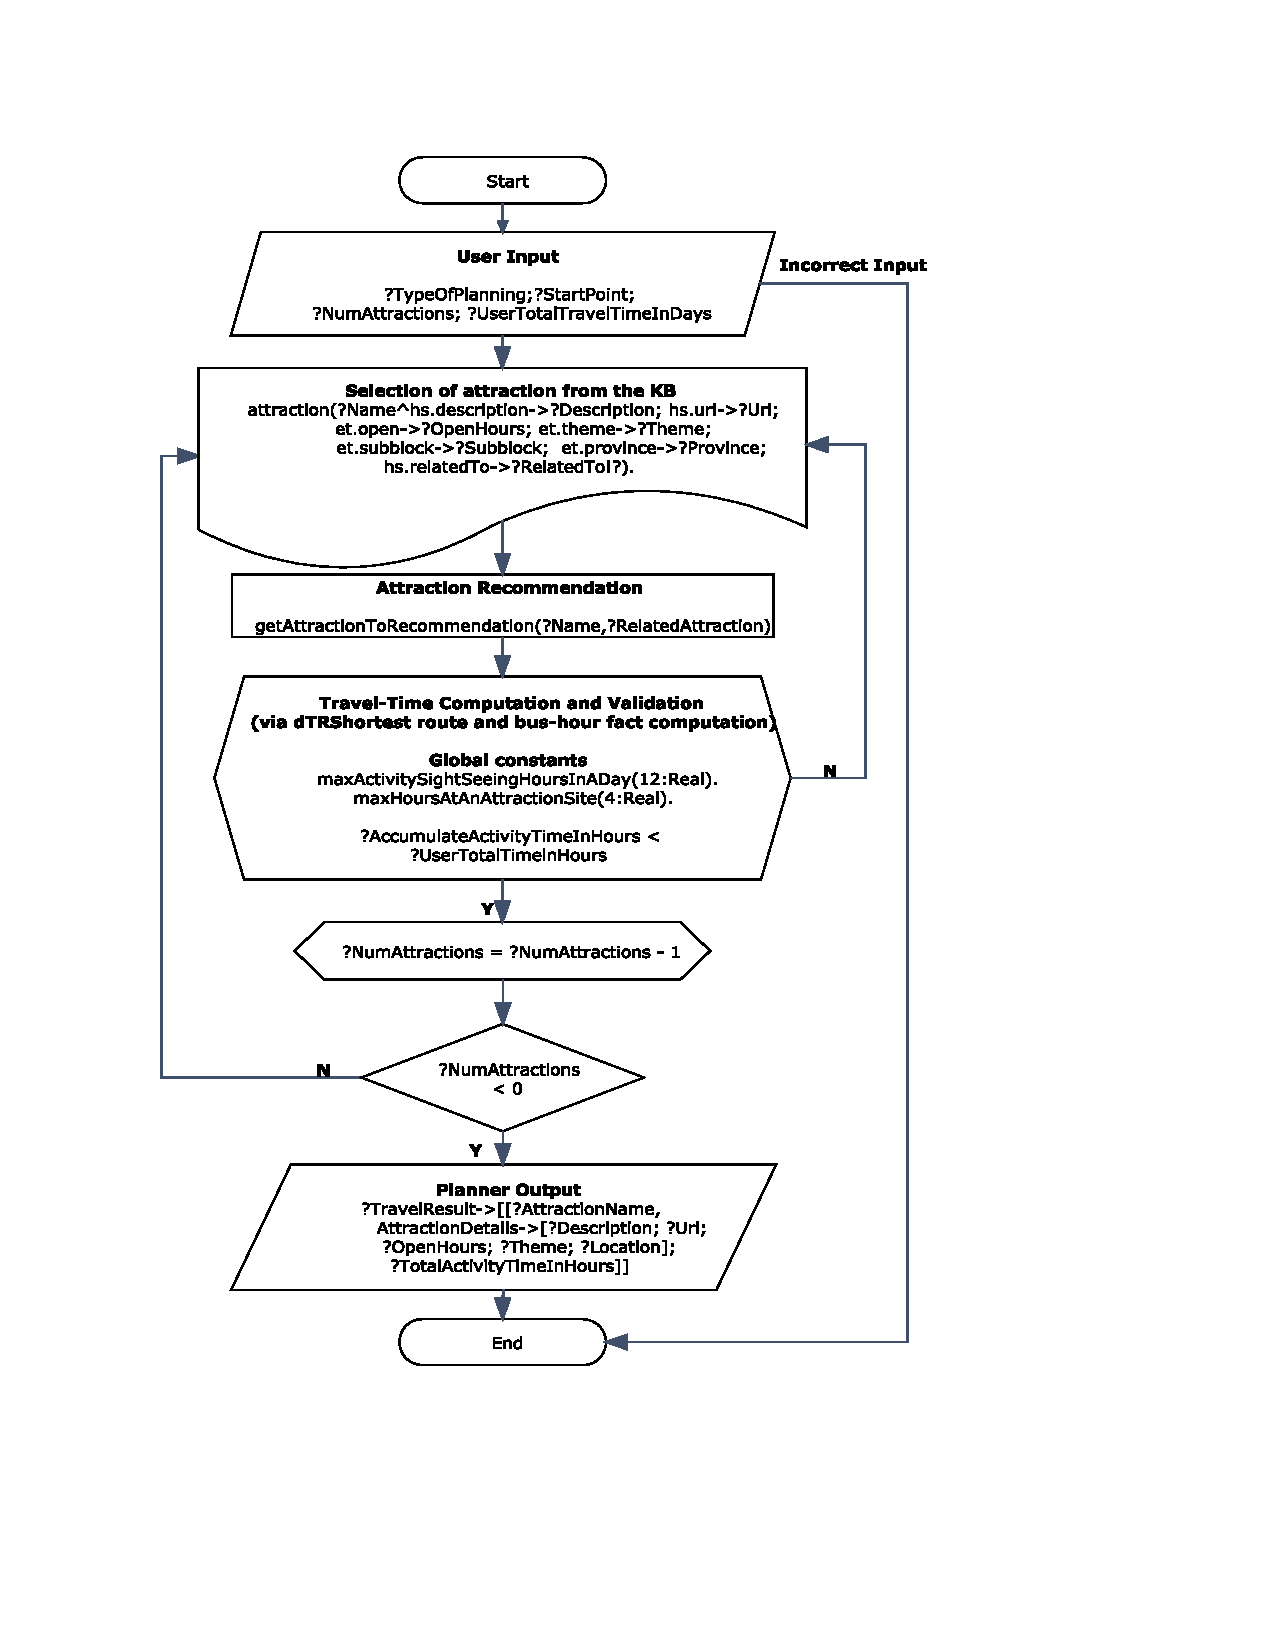
\includegraphics[width=5.5in, height=8.3in]{eTourPlanA}
\caption {The top-level of attraction-only planning}
\label{fig:Fig5.5}
\end{center}
\end{figure} 
					  
Users must input the following slot fillers: 
\singlespacing
\begin{itemize}
\item ?TypeOfPlanning: AttractionOnly
\item ?StartPoint: Starting province
\item ?NumAttractions: Number of attractions to be included in the plan  
\item ?UserTotalTravelTimeInDays: Users total travel time in days
\end{itemize}

The system outputs the following slot fillers:
\begin{itemize}
\item ?AttractionList: List of attractions to visit
\item ?TotalActivityTimeInHours: Actual total time of the tour
\end{itemize}

\doublespacing
The planner performs the following steps in sequence:
\begin{itemize}
\item From the user-specified starting point, an attraction is selected and chains to the
next related attraction.
\item Compute and validate route and
travel-time constrained by global
constants: 
\begin{itemize}
\item maxActivitySightSeeingHoursInADay(12:Real).
\item maxHoursAtAnAttractionSite(4:Real).
\end{itemize}
\item On successful validation of distance and
remaining time, add detailed information
of the selected attraction to the travel
plan.
\end{itemize}

A sample query of the top-level eTourPlan attraction-only rule system is shown below:
\\ 
\begin{small}
    \textbf{Sample Query}
\end{small}

\begin{small}
\singlespacing
\begin{verbatim}
eTourPlan(typeOfPlanning->AttractionOnly;
          userInputs->[startPoint->Bumthang:Province;
                       numAttractions->4:Integer;
                       userTotalTravelTimeInDays->3:Real];
          travelResult->?TravelPlan)
\end{verbatim}
\end{small}   

The solution for the above eTourPlan query:
\\
\begin{small}
    \textbf{OO jDREW TD Result}
\end{small}

\begin{small}
\singlespacing
\begin{verbatim}
?TravelPlan=
	[[[Bumthang_Dzong:Fortress; 
       AttractionDetails->[
          Description->"The Bumthang Dzong or the Dzong of the white bird. 
                       It is perched on the hillock over looking Chamkhar 
                       town & places surrounding it. The interesting thing 
                       about the Dzong is, that there is a water tower four 
                       stairs down behind the Dzong."; 
          Url->" ";
          OpenHours->9amTo4pm;
          Theme->Cultural_Religious_Heritage;
          Location->[Chamkhar:Town, Bumthang:Province]]], 
																			
		[Samchholing_Palace:Popular_architecture;
       AttractionDetails->[
          Description->"Samchholing was built by the Second King. It was 
                        later handed over to Ashi Pem Dechen, mother of 
                        HRH Namgyel Wangchuck. It is about to be in ruins, 
                        but it has a beautiful architecture."; 
          Url->" ";
          OpenHours->9amTo4pm; 
          Theme->Cultural_Religious_Heritage; 
          Location->[Samcholing:Village, Trongsa:Province]]], 
			  
		 [Trongsa_Dzong:Fortress;
        AttractionDetails->[
           Description->"It was built by Zhabdrung Rimpochhe. It is one of 
                         the biggest fortress in Bhutan";
           Url->" ";
           OpenHours->9amTo4pm;
           Theme->Cultural_Religious_Heritage;
           Location->[Samcholing:Village, Trongsa:Province]]],

		 Wangdue_Dzong:Fortress; 
		   AttractionDetails->[
		      Description->"It is one of the most beautiful attractions in the
		                    Southern region"; 
		      Url->" "; 
		      OpenHours->9amTo4pm;
		      Theme->Cultural_Religious_Heritage;
          Location->[Wangdue_Town:Town, WangduePhodrang:Province]]]; 
					  
		 TotalActivityTimeInHours->26.0:Real]			   
\end{verbatim}
\end{small} 

\subsection{eTourPlan Event-Centric Planning}

\hspace{0.3in}The event-centric planning takes into account the time constraint of event dates, in accordance to the user's preferred time frame for a vacation. We perform the selection of events by date validation, followed by the validation of distance between the event locations. The planner recommends attractions that are located in the subblock of each selected event. An additional option for on-route attraction recommendation is also provided. In a similar manner, we could integrate the accommodation search predicate discussed in Section 5.2.3.3, to provide accommodation recommendation in each of the event-containing subblocks. 

\begin{figure}
\begin{flushleft}
    \textbf{\large eTourPlan Event-Centric}
\end{flushleft}
\begin{center}
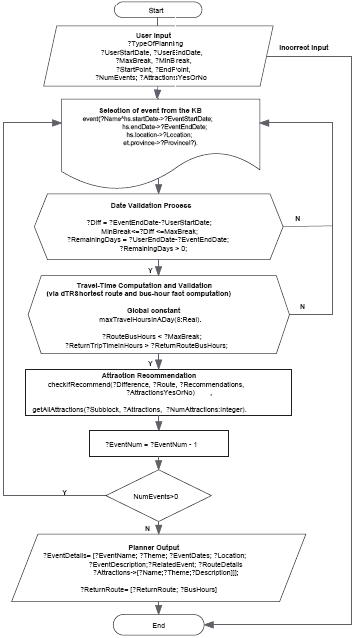
\includegraphics[width=5.5in, height=8.3in]{eTourPlanE}
\caption {The top-level of event-centric planning}
\label{fig:Fig5.5}
\end{center}
\end{figure}

The eTourplan event-centric planner considers the following needs and constraints of users:
\begin{itemize}
\item\textbf{Preferences}: Users would have their preference of time for making a trip. For instance, a tourist might want to take a month's vacation in February. Users can provide preferences for the attraction theme and type of accommodation to be recommended.

\item \textbf{Constraints}: Maximum break between events: This is considered as the upper bound on the break (time)
between two events. This is also considered as the maximum travel time between two event locations for a particular user in the context of this thesis. The second constraint is the minimum break, which is the lower bound on the break between events. Many users would not mind experiencing two events on two consecutive days but we are still allowing users to specify the minimum break between events for flexibility. 
\end{itemize}

\hspace{0.3in}The event-centric planner generates the travel plan by selecting a specified number of N events between the  user's specified travel dates. The rule system mainly validates the time and distance of each event. The flowchart in Figure 5.7 illustrates the top-level event planning strategy. The complete system is given in Appendix A.\\

Users must input the following slots: 
\singlespacing
\begin{itemize}
 \item ?UserStartDate: User's preferred start date of travel
 \item ?UserEndDate:  User's preferred end date of travel
 \item ?StartProvince: Start point of the travel
 \item ?EndProvince: End point of the travel
 \item ?MaxBreak: Maximum break between events
 \item ?MinBreak: Minimum break between events
 \item ?NumEvents: Number of events to be included in the plan  
 \item ?AttractionYesOrNo: User selects the optional on-route attraction recommendation
\end{itemize}
The system outputs the following slots:
\begin{itemize}
 \item ?EventDetails: Detail information for each selected event with route information
 \item ?ReturnRoute:  Route and distance time to the specifed EndProvince      
\end{itemize} 

\doublespacing

\hspace{0.3in}The planner performs the following steps in sequence:
\begin{itemize}
\item Events are selected by validating the event dates
against the user�s travel dates, minimum break,
and maximum break.
\item Compute and validate route and bus hours between event locations constrained by the specified maximum break.
\item On successful validation of distance and
remaining time, add detailed information of the
selected event to the travel plan.
\item Recommend attractions located in the subblock
of the selected event.
\item Provide on-route attraction recommendation if
the user selects the option (constrained by the
global constant �maxTimeGapBetweenEvents").
\end{itemize}

\hspace{0.3in}A sample query for the top-level event-centric eTourPlan rule system is shown below. The planner generates an event tour for a given time frame based on the needs and constraints provided by the user.
\\

\begin{small}
    \textbf{Sample Query}
\end{small}
\begin{small}
\singlespacing
\begin{verbatim}
 eTourPlan(typeOfPlanning->EventCentric; 
           userInputs->[userStartDate->date[2008:Real, 10:Real, 01:Real]; 
                        userEndDate->date[2008:Real, 11:Real, 10:Real];
                        maxBreak->11:Real;  
                        minBreak->0:Real;  
                        startPoint->Paro:Province;  
                        endPoint->Thimphu:Province;
                        attractionRecommendation->Yes; 
                        eventNum->1:Integer];
           ?TravelResult)        
\end{verbatim}
\end{small}   
A sample solution for the above eTourPlan query is shown below:
\\
\begin{small}
    \textbf{OO jDREW TD Result}
\end{small}

\begin{small}
\singlespacing
\begin{verbatim}
?TravelResult=
	[[[EventName->Thimphu_Tshechu:Annual_festival;
     EventDates->[Startdate->date[2008:Real, 10:Real, 09:Real];
                  Enddate->date[2008:Real, 10:Real, 11:Real]];
     Theme->Cultural_Religious_Heritage;
     Location->[Tashichoe_Dzong:Fortress,
                Jongshina:Town,
                Thimphu:Province];
     EventDescription->"It is a popular festival in Thimphu";
     RelatedEvents->Tangbi_Mani:Traditional_festival;
     RouteDetails->[
      [Paro:Province, Chuzom:Province, Thimphu:Province];  
       RouteBusHours->4.5:Real;
       RecommendedAttractions->[
        [Paro:Province;
          Attraction->[AttractionName->Rinpung_Dzong:Fortress;
                       RelatedTo->Taktshang:Monastery;
                       Theme->Cultural_Religious_Heritage;
                       Subblock->Phatsana:Village]],

        [Chuzom:Province; 
          Attraction->[]],
        [Thimphu:Province;
          Attraction->[AttractionName->Tashichoe_Dzong:Fortress;
                       RelatedTo->"Memorial_Chorten:Temple";
                       Theme->Cultural_Religious_Heritage;
                       Subblock->Jongshina:Town]]]]]];
  ReturnRoute->[[Thimphu:Province]; Returntime->0:Real]]       			   
\end{verbatim}
\end{small} 

\hspace{0.3in}The system finds three events from the KB, one at a time, each one of which is validated w.r.t. time and distance. The planner offers three different events occurring at different dates between the user-specified travel dates. The planner also provides on-route attraction recommendations if the time gap between the event dates is more than five days (global constant ``maxTimeGapBetweenEvents"). Setting ``eventNum" to 3 in the above query will go travel plans consisting of alternative combinations of three events with respect to thier times and distances. The complete eTourPlan planning rule system is given in Appendix A.
%\\
%\begin{small}
 %   \textbf{Sample Query}
%\end{small}

\hspace{0.3in} Attraction recommendations can be done at any level of the partonomy. In this thesis, attractions can be recommended both at the province and the subblock level, but we have tested the prototype with attraction recommendations at the subblock level to obtain maximum granularity. Similarly, accommodation recommendation at any level of the partonomy can be integrated as another optional feature into the planner. The integration of recommendations for routes, attractions, and accommodations into the event-centric planning amounts to packaging a complete travel for users. 




